% ========================================= TEMPLATE INFO ========================================
%
% Author:       P4ntomime
% Version:      1.0.0
% Last updated: 2024-02-18
% Brief:        A LaTeX template for summaries. See README.md for more information.
% 
% ================================================================================================
\documentclass[8pt, a4paper, twoside]{extarticle}
% Font size:    8pt
% Paper size:   A4
% style:        twoside (needed, so odd and even pages have different margins)
% orientation:  portrait. (use 'landscape' for landscape orientation)


% ========================================= DOCUMENT INFO =========================================
\def\title{Energiesysteme}           % title
\def\shorttitle{EnSys} % short title (displayed as PDF title)
\def\dozent{Dr. A Fuchs, Dr. T Demiray}         % lecturer
\def\semester{6. Semester}     % semester
\def\author{Luca Loop}        % author(s)
\def\repo{https://github.com/Luca-ET/EnSys.git}             % repository link
\def\version{1.0.\today}    % version
\def\pagelimit{100}           % page limit -> causes pages after limit to be red
\def\titleoption{compact}   % options: ultra compact, compact, normal
\def\enableToC{true}

% ================================= PACKAGES, SETUP AND COMMANDS ==================================
% =========================================== PACKAGES ============================================
\usepackage[utf8]{inputenc}         % input encoding: UTF-8
\usepackage[T1]{fontenc}            % font encoding: T1
\usepackage{textcomp}               % additional symbols
\usepackage{times}                  % times new roman font
\usepackage{inconsolata}            % inconsolata font for listings
\usepackage[main=ngerman]{babel}    % set main language to german


\usepackage{multicol}               % provides multicols environment
\usepackage{geometry}               % set page layout


\usepackage{enumitem}               % list customization
\usepackage{outlines}               % easy nested lists
\usepackage{tabularx}               % some nicer tables with X columns
\usepackage{tabu}                   % more flexible tables
\usepackage{hhline}                 % double lines in tables
\usepackage{booktabs}               % thick and thin lines in tables
\usepackage{boldline}               % bold (vertical) lines in tables


\usepackage{amsmath}                % math symbols
\usepackage{amssymb}                % more math symbols
\usepackage{mathtools}              % more math tools needed for pmatrix modification
\usepackage{mhsetup}                % needed to modify pmatrix environment
\usepackage{txfonts}                % Times math font
\usepackage[squaren]{SIunits}       % SI-units
\usepackage{bm}                     % bold math symbols
\usepackage{trfsigns}               % needed for "Laplace" symbol (Korrespondenz)
\usepackage{mathrsfs}               % needed for Fourier transform "F"



\usepackage{graphicx}               % include graphics
\usepackage{graphbox}               % needed for aligning images in multicol environment
\usepackage{scalerel}               % scale any objects
\usepackage{anyfontsize}            % set any font size
\usepackage[table]{xcolor}          % needed for colors


\usepackage{tcolorbox}              % colored boxes
\usepackage[outline]{contour}       % contour for text (used in custom underline command)
\usepackage[normalem]{ulem}         % custom underline (used in custom underline command)


\usepackage{tikz}                   % needed for TikZ drawings
\usepackage{pgfplots}               % Draw nice plots


\usepackage{listings}               % for nicer code display
% to use nodes inside listing see: https://texample.net/tikz/examples/tikz-listings/


\usepackage{hyperref}               % clickable links
\usepackage{qrcode}                 % QR code generation (also clickable)


\usepackage{ifthen}                 % if-then-else commands
\usepackage{calc}                   % simple arithmetic in LaTeX commands


\usepackage{draftwatermark}         % watermark on pages after a certain limit
\usepackage{fancyhdr}               % custom header and footer
\usepackage[explicit]{titlesec}     % custom section titles


\usepackage{datetime2}              % custom date format for versioning


% ========================================== BASIC SETUP ==========================================

% --------------------------------------- DOCUMENT SETTINGS ---------------------------------------
\hypersetup{hidelinks,
% set pdf metadata
            pdfauthor={\author},
            pdftitle={\shorttitle},
            pdfsubject={\title\ \semester},
            pdfkeywords={Gahn go lerne!!}}

% set style for URLs
\urlstyle{same} % sets url font to the same as the preceeding text

% set page layout
\geometry{left=3mm, 
          right=3mm, 
          top=3mm, 
          bottom=6mm, 
          headheight=0mm, 
          headsep=0mm, 
          footskip=4mm,
        %   showframe,
          }

\setlength{\columnsep}{1.5mm}       % distance between columns
\setlength{\columnseprule}{0.1pt}   % thickness of column separation line
\setlength{\parindent}{0pt}         % no paragraph indentation

\setcounter{tocdepth}{2}            % only display sections and subsections in toc
% \setcounter{secnumdepth}{0}       % uncomment to disable section numbering

\DeclareMathSizes{8}{8}{6}{5}       % set math font sizes for 8pt document


% --------------------------------------- COLOR DEFINITIONS ---------------------------------------
\definecolor{sectioncolor}{HTML}{ffff00}
\definecolor{subsectioncolor}{HTML}{ffff99}
\definecolor{sectextcol}{HTML}{000000}
\definecolor{subsectextcol}{HTML}{000000}

\definecolor{backcolour}{HTML}{f5f5f0} % background color for highlighted text

% TODO: define color palette
% color palette: https://colorkit.co/color-palette-generator/FF8552-9e22bd-404E7C-C32E15-225A28/
\definecolor{green}{HTML}{1af430}
\definecolor{red}{HTML}{f90d09}
\definecolor{blue}{HTML}{093ce5}
\definecolor{orange}{HTML}{f7730e}
\definecolor{violet}{HTML}{a516c9}

% colors for listings (code)
\definecolor{commentcolour}{HTML}{6a9955}
\definecolor{keywordcolour}{HTML}{7f0055}
\definecolor{stringcolour}{HTML}{9e22bd}
\definecolor{numbercolour}{HTML}{808080}


% ----------------------------------- LIST AND TABULAR SETTINGS -----------------------------------
\setlist[enumerate]{%
    labelindent=0pt,                                % no indentation for labels
    labelwidth = \widthof{\ref{enum-\EnumitemId}},  % set label width to widest label
    label=\bfseries\arabic*.,                       % label style bold arabic numerals (1., 2., ...)
    itemindent=1ex,                                 % separation between label and item text
    leftmargin=!,                                   % automatically calculate left margin
    after=\label{enum-\EnumitemId}}                 % set label for referencing in labelwidth

\setlist[itemize]{leftmargin=1.5em}                 % left margin for itemize: 1.5em
\setlist[description]{leftmargin=2ex}               % left margin for description: 2ex
\setlist{nosep}                                     % no vertical spacing between list items

\renewcommand{\arraystretch}{1}                     % stretch table rows

\setcounter{MaxMatrixCols}{32}                      % increase max columns in matrix environments

% ----------------------------------- TIKZ & PGF-PLOTS SETTINGS -----------------------------------
\usetikzlibrary{arrows}
\usetikzlibrary{arrows.meta}
\usetikzlibrary{bending}
\usetikzlibrary{decorations.pathreplacing}
\usetikzlibrary{angles}
\usetikzlibrary{tikzmark}
\usetikzlibrary{petri}
\usetikzlibrary{positioning}
\usetikzlibrary{shapes}
\usetikzlibrary{calc}

\pgfplotsset{compat=1.18}

% ------------------------------------ OTHER PACKAGE SETTINGS -------------------------------------

% define and set new date style for versioning as YYYYMMDD
\DTMnewdatestyle{vnumdate}{%
    \renewcommand{\DTMdisplaydate}[4]{\number##1\DTMtwodigits{##2}\DTMtwodigits{##3}}%
    \renewcommand{\DTMDisplaydate}{\DTMdisplaydate}%
}
\DTMsetdatestyle{vnumdate}


% setup for ulem and contour packages
\renewcommand{\ULdepth}{1.75pt} % set underline depth
\contourlength{0.7pt}           % set contour length


% ====================================== SETUP AND COMMANDS =======================================

% custom font size for paragraph titles
\newcommand{\semilarge}{\fontsize{9}{8}\selectfont} % new font size \semilarge (9pt)

\ExplSyntaxOn
% custom underline command for exclusions on lowercase letters such as g, j, p, q, y
\newrobustcmd{\myul}[1]{%
    \if_mode_math:
        \text{%
            \uline{\phantom{$#1$}}%
            \llap{\contour{white}{$#1$}}%
        }
    \else:
        \uline{\phantom{#1}}%
        \llap{\contour{white}{#1}}%
    \fi:
}

\renewrobustcmd{\underline}[1]{%
    \if_mode_math:
        \text{%
            \uline{\phantom{$#1$}}%
            \llap{\contour{white}{$#1$}}%
        }
    \else:
        \uline{\phantom{#1}}%
        \llap{\contour{white}{#1}}%
    \fi:
}
\ExplSyntaxOff


% setup header and footer
\pagestyle{fancy}
\fancyhf{}                          % clear all header and footer fields
\renewcommand{\headrulewidth}{0pt}  % remove header rule
\renewcommand{\footrulewidth}{0pt}  % remove footer rule
\fancyfoot[C]{\thepage}             % page number in center of footer


% --------------------------------------- TITLE FORMATTING ----------------------------------------

\titleclass{\part}{straight}

% part formatting
\titleformat{\part}
            {\huge\bfseries}
            {\thepart}
            {1em}
            {#1}

\titlespacing{\part}
             {0.6ex}
             {1ex}
             {1ex}

% section formatting
\titleformat{\section}
            % {\fontsize{9}{8}\selectfont\bfseries}
            {\Large\bfseries}
            {}
            {0mm}
            {\tikz{
                \node[fill=sectioncolor,            % fill color:       sectioncolor
                      text=sectextcol,              % text color:       sectextcol
                      text width=\columnwidth-4pt,  % text width:       columnwidth - 2x padding
                      text depth=0pt,               % text depth:       0pt (needed so text stays vertically centered)
                      minimum height=5mm,           % minimum height:   5mm
                      inner sep=2pt,                % inner padding:    2pt
                      align=left]                   % text alignment:   left
                      {\thesection\ #1};}}

\titleformat{numberless, name=\section}
            % {\fontsize{9}{8}\selectfont\bfseries}
            {\Large\bfseries}
            {}
            {0mm}
            {\tikz{
                \node[fill=sectioncolor,            % fill color:       sectioncolor
                      text=sectextcol,              % text color:       sectextcol
                      text width=\columnwidth-4pt,  % text width:       columnwidth - 2x padding
                      text depth=0pt,               % text depth:       0pt (needed so text stays vertically centered)
                      minimum height=5mm,           % minimum height:   5mm
                      inner sep=2pt,                % inner padding:    2pt
                      align=left]                   % text alignment:   left
                      {#1};}}

\titlespacing{\section}
             {0mm}
             {.2ex}
             {.2ex}


% subsection formatting
\titleformat{\subsection}
            {\large\bfseries}
            {}
            {0mm}
            {\phantomsection\tikz{
                \node[fill=subsectioncolor,         % fill color:       subsectioncolor 
                      text=subsectextcol,           % text color:       subsectextcol 
                      text width=\columnwidth-4pt,  % text width:       columnwidth - 2x padding 
                      text depth=0pt,               % text depth:       0pt (needed so text stays vertically centered)
                      minimum height=5mm,           % minimum height:   5mm 
                      inner sep=2pt,                % inner padding:    2pt 
                      align=left]                   % text alignment:   left
                      {\thesubsection\ #1};}}

\titleformat{numberless, name=\subsection}
            {\large\bfseries}
            {}
            {0mm}
            {\phantomsection\tikz{
                \node[fill=subsectioncolor,         % fill color:       subsectioncolor 
                      text=subsectextcol,           % text color:       subsectextcol 
                      text width=\columnwidth-4pt,  % text width:       columnwidth - 2x padding 
                      minimum height=5mm,           % minimum height:   5mm 
                      inner sep=2pt,                % inner padding:    2pt 
                      align=left]                   % text alignment:   left
                      {#1};}}

\titlespacing{\subsection}
             {0mm}
             {1ex}
             {.2ex}


% subsubsection formatting
\titleformat{\subsubsection}
            {\large\bfseries}
            {\myul{\thesubsubsection\ }}
            {0mm}
            {\phantomsection{}\myul{#1}}

\titlespacing{\subsubsection}
             {0mm}
             {1ex}
             {1ex}


% paragraph formatting
\titleformat{\paragraph}[runin]
            {\semilarge\bfseries}
            {}
            {0mm}
            {#1\normalfont :\;}

\titlespacing{\paragraph}
             {0mm}
             {0ex}
             {0.1ex}


% new alias for paragraph '\para' (shorter than \paragraph)
\let\para\paragraph%

% custom command for examples
\newcommand{\example}[1]{\subsubsection*{Beispiel: #1}}


% ----------------------------------- CUSTOM TABULAR SPECIFIERS -----------------------------------

% centered fixed width column type
\newcolumntype{P}[1]{>{\centering\arraybackslash}p{#1}}

 % centered variable width column type
\newcolumntype{C}{>{\centering\arraybackslash}X}

% centered math column type
\newcolumntype{M}{>{$}c<{$}}


% inline tikz node for later referencing
\newcommand{\tikznode}[2]{% from https://tex.stackexchange.com/a/402466/121799
	\ifmmode%
	\tikz[remember picture,baseline= (#1.base),inner sep=0pt] \node(#1){$#2$};
	\else
	\tikz[remember picture,baseline= (#1.base),inner sep=0pt] \node(#1){#2};
	\fi}


% custom inline tcolorbox
\newtcbox{\mybox}
            [1]
            [backcolour]
            {on line,
            arc=0pt,
            outer arc=0pt,
            colback=#1,
            colframe=#1,
            boxsep=0pt,
            left=1pt,
            right=1pt,
            top=1pt,
            bottom=1pt,
            boxrule=0pt}


\makeatletter

% ------------------------------- SECTIONING COMMANDS CUSTOMIZATION -------------------------------

% section: add optional argument to command for script page numbers
\let\old@sec\section%
\RenewDocumentCommand{\section}{somg}{%
    \IfBooleanTF{#1}{
        \IfNoValueTF{#2}{
            \IfNoValueTF{#4}{
                \old@sec*{#3}
            }{
                \old@sec*{#3 {\small(S. #4)}}
            }
        }{
            \IfNoValueTF{#4}{
                \old@sec*[#2]{#3}
            }{
                \old@sec*[#2]{#3 {\small(S. #4)}}
            }
        }%
    }{
        \IfNoValueTF{#2}{
            \IfNoValueTF{#4}{
                \old@sec{#3}
            }{
                \old@sec{#3 {\small(S. #4)}}
            }
        }{
            \IfNoValueTF{#4}{
                \old@sec[#2]{#3}
            }{
                \old@sec[#2]{#3 {\small(S. #4)}}
            }
        }%
    }
}


% subsection: add optional argument to command for script page numbers
\let\old@subsec\subsection%
\RenewDocumentCommand{\subsection}{somg}{%
    \IfBooleanTF{#1}{
        \IfNoValueTF{#2}{
            \IfNoValueTF{#4}{
                \old@subsec*{#3}
            }{
                \old@subsec*{#3 {\small(S. #4)}}
            }
        }{
            \IfNoValueTF{#4}{
                \old@subsec*[#2]{#3}
            }{
                \old@subsec*[#2]{#3 {\small(S. #4)}}
            }
        }%
    }{
        \IfNoValueTF{#2}{
            \IfNoValueTF{#4}{
                \old@subsec{#3}
            }{
                \old@subsec{#3 {\small(S. #4)}}
            }
        }{
            \IfNoValueTF{#4}{
                \old@subsec[#2]{#3}
            }{
                \old@subsec[#2]{#3 {\small(S. #4)}}
            }
        }%
    }
}


% subsubsection: add optional argument to command for script page numbers
\let\old@subsubsec\subsubsection%
\RenewDocumentCommand{\subsubsection}{somg}{%
    \IfBooleanTF{#1}{
        \IfNoValueTF{#2}{
            \IfNoValueTF{#4}{
                \old@subsubsec*{#3}
            }{
                \old@subsubsec*{#3 {\small(S. #4)}}
            }
        }{
            \IfNoValueTF{#4}{
                \old@subsubsec*[#2]{#3}
            }{
                \old@subsubsec*[#2]{#3 {\small(S. #4)}}
            }
        }%
    }{
        \IfNoValueTF{#2}{
            \IfNoValueTF{#4}{
                \old@subsubsec{#3}
            }{
                \old@subsubsec{#3 {\small(S. #4)}}
            }
        }{
            \IfNoValueTF{#4}{
                \old@subsubsec[#2]{#3}
            }{
                \old@subsubsec[#2]{#3 {\small(S. #4)}}
            }
        }%
    }
}


% custom text rightarrow to match tikz arrows
\renewrobustcmd{\textrightarrow}{%
    \raisebox{0.2ex}{%
        \tikz[line width=0.11ex, >={Stealth[length=1.1ex, inset=0.2ex]}]{%
            \draw (0,-0.13ex) to (0.55em, -0.13ex);%
            \draw (0, 0.13ex) to (0.55em,  0.13ex);%
            \draw[line width=0pt, ->] (0.8em,0) to (0.9em,0);%
        }%
    }%
}%

% custom text leftrightarrow to match tikz arrows
\newrobustcmd{\textlrarrow}{%
    \raisebox{0.2ex}{%
        \tikz[line width=0.11ex, >={Stealth[length=1.1ex, inset=0.2ex]}]{%
            \draw (0.35em,-0.13ex) to (0.9em, -0.13ex);%
            \draw (0.35em, 0.13ex) to (0.9em,  0.13ex);%
            \draw[line width=0pt, ->] (1.15em,0) to (1.25em,0);%
            \draw[line width=0pt, <-] (0,0) to (0.1em,0);%
        }%
    }%
}%


% renews the pmatrix environment to use \lgroup and \rgroup instead of \left( and \right)
\renewenvironment{pmatrix}{%
    \left\lgroup%
    \matrix@check\pmatrix\env@matrix%
}{
    \endmatrix\right\rgroup%
}

% renews the pmatrix* environment to use \lgroup and \rgroup instead of \left( and \right)
\MHInternalSyntaxOn%
\renewenvironment{pmatrix*}[1][c]
  {\left\lgroup\MT_matrix_begin:N #1}
  {\MT_matrix_end:\right\rgroup}
\MHInternalSyntaxOff%


% new environment for centered tabulars
\NewDocumentEnvironment{ctabular}{m}
                        {\center\tabular{#1}}
                        {\endtabular\endcenter}


% custom command for size matched colored brackets
\newcommand{\bbr}[2]{\colorlet{saved}{.}\color{#1}\left(\color{saved}#2\color{#1}\right)\color{saved}}


% custom command for differential operator d
\newcommand{\diff}{\ensuremath{\mathop{} \! \mathrm{d}}}
\newcommand{\dd}{\diff}


% custom command for underset limes operator
\newcommand{\limes}[1]{\ensuremath{\underset{#1}{\lim}}}

% custom command for absolute value
\newcommand{\abs}[1]{\ensuremath{\left|#1\right|}}


% shortcuts for colored text
\newcommand{\cgn}[1]{{\color{green}#1}}
\newcommand{\crd}[1]{{\color{red}#1}}
\newcommand{\cbl}[1]{{\color{blue}#1}}
\newcommand{\cor}[1]{{\color{orange}#1}}
\newcommand{\cvt}[1]{{\color{violet}#1}}


% bullet command for items in tables
\newcommand{\tabitem}{~~\llap{\textbullet}~~}


% customizes watermark and page color after a certain page limit
% colors all pages after the specified limit red
% source: https://stackoverflow.com/questions/2720534/force-a-maximum-number-of-pages-in-latex 
\newcounter{page@count}
\setcounter{page@count}{0}
\gdef\maxpages{\pagelimit}
\ifx\latex@outputpage\@undefined\relax% ChkTeX 21
    \global\let\latex@outputpage\@outputpage% ChkTeX 21
\fi%
\gdef\@outputpage{% ChkTeX 21
    \addtocounter{page@count}{1}%
    \ifnum\value{page@count}>\maxpages\relax%
        % change page background to red and add watermark
        \SetWatermarkText{\pagelimit\ Seiten Limit erreicht!}%
        \SetWatermarkScale{0.35}%
        \pagecolor{red}
        \latex@outputpage%
    \else%
        \SetWatermarkText{}%
        \latex@outputpage%
    \fi%
}


% remove title from table of contents, needed for layout
\renewcommand{\tableofcontents}{%
    \@starttoc{toc}
}


% scale super- and subscript -- not used currently, instead resized math font
% \catcode`_=\active% chktex 41 --> suppress ChkTeX warning
% \catcode`^=\active% chktex 41
% \newcommand_[1]{\ensuremath{\sb{\mathrm{\scaleobj{0.7}{#1}}}}}
% \newcommand^[1]{\ensuremath{\sp{\mathrm{\scaleobj{0.7}{#1}}}}}


\makeatother


% new environment for layout --> automatically adjusts to landscape or portrait
\ExplSyntaxOn
\NewDocumentEnvironment{layout}{}{
    \dim_compare:nNnT{\paperwidth}<{\paperheight}
    {
        % PORTRAIT LAYOUT
        \str_case:en{\str_lowercase:f\titleoption}
        {
            {ultra~compact}
            {
                \str_if_eq:eeTF {\str_lowercase:f\enableToC}{true}
                {
                    \begin{minipage}[t]{0.1\columnwidth} % DigDes-like formatting
                        \raisebox{-.3\columnwidth}{\qrcode[level=L, 
                                version=0,
                                height=0.9\columnwidth]{\repo}}\hfill
                        \normalfont\footnotesize\rotatebox[origin=tr]{90}{V \version{}}
                    \end{minipage}\hfill
                    \begin{minipage}[t]{0.89\columnwidth}
                        \raggedright%
                        \normalfont\Huge\bfseries\title{}\\[1mm]
                        \normalfont\Large\semester\ --\ \dozent{}\\
                        \large Autoren:\ \author{}\\[1mm]
                        \myul{\url{\repo}}
                    \end{minipage}\par
                        \section*{\contentsname}
                        \group_begin:
                        \setlength{\columnsep}{5mm}
                        \begin{multicols}{2}
                            \tableofcontents%
                        \end{multicols}
                        \group_end:
                        \hrule
                    \begin{multicols*}{2}
                    \raggedcolumns%
                }
                {
                    \begin{multicols*}{2}
                    \raggedcolumns%
                    \begin{minipage}[t]{0.2\columnwidth} % MathFML-like formatting
                        \vspace{-0.225\columnwidth}
                        \qrcode[level=L, 
                                version=0,
                                height=0.9\columnwidth]{\repo}\hfill
                        \normalfont\footnotesize\rotatebox[origin=tr]{90}{V \version{}}
                    \end{minipage}\hfill
                    \begin{minipage}[t]{0.79\columnwidth}
                        \raggedright%
                        \normalfont\Huge\bfseries\title{}\\[1mm]
                        \normalfont\Large\semester\ --\ \dozent{}\\
                        \large Autoren:\ \author{}\\[1mm]
                        \normalsize\myul{\url{\repo}}
                    \end{minipage}\par
                }
            }
            {compact}
            {
                \str_if_eq:eeTF {\str_lowercase:f\enableToC}{true}
                {
                    \begin{minipage}[t]{0.1\columnwidth} % Elo-like formatting
                        \raisebox{-.3\columnwidth}{\qrcode[level=L, 
                                version=0,
                                height=0.9\columnwidth]{\repo}}\hfill
                        \normalfont\footnotesize\rotatebox[origin=tr]{90}{V \version{}}
                    \end{minipage}\hfill
                    \begin{minipage}[t]{0.89\columnwidth}
                        \raggedright%
                        \normalfont\Huge\bfseries\title{}\\[1mm]
                        \normalfont\Large\semester\ --\ \dozent{}\\
                        \large Autoren:\ \author{}\\[1mm]
                        \myul{\url{\repo}}
                    \end{minipage}\par
                    \section*{\contentsname}
                    \group_begin:
                    \setlength{\columnsep}{5mm}
                    \begin{multicols}{2}
                        \tableofcontents%
                    \end{multicols}
                    \group_end:
                    \vfill
                    \newpage
                    \begin{multicols*}{2}
                    \raggedcolumns%
                }
                {
                    \begin{multicols*}{2}
                    \raggedcolumns%
                    \begin{minipage}[t]{0.2\columnwidth} % MathFML-like formatting
                        \vspace{-0.225\columnwidth}
                        \qrcode[level=L, 
                                version=0,
                                height=0.9\columnwidth]{\repo}\hfill
                        \normalfont\footnotesize\rotatebox[origin=tr]{90}{V \version{}}
                    \end{minipage}\hfill
                    \begin{minipage}[t]{0.79\columnwidth}
                        \raggedright%
                        \normalfont\Huge\bfseries\title{}\\[1mm]
                        \normalfont\Large\semester\ --\ \dozent{}\\
                        \large Autoren:\ \author{}\\[1mm]
                        \normalsize\myul{\url{\repo}}
                    \end{minipage}\par
                }
            }
            {normal}
            {
                \hfill\null\vspace{1cm}
                \begin{center}
                    \normalfont\fontsize{35}{32}\selectfont\bfseries\title{}\\[7.5mm]
                    \normalfont\huge\semester\ --\ \dozent{}\\
                    \Large Autoren:\\
                    \Large\author{}\\[2mm]
                    \large Version:\\
                    \large\version{}\\
                    \normalsize\myul{\url{\repo}}\\[2mm]
                    \qrcode[level=L, 
                            version=0,
                            height=2cm]{\repo}
                \end{center}
                \vfill
                \thispagestyle{empty}
                \str_if_eq:eeT {\str_lowercase:f\enableToC}{true}
                {
                    \section*{\contentsname}
                    \group_begin:
                    \setlength{\columnsep}{5mm}
                    \begin{multicols}{2}
                        \tableofcontents%
                    \end{multicols}
                    \group_end:
                    \vfill
                }
                \newpage
                \begin{multicols*}{2}
                \raggedcolumns%
            }
        }
    }
    
    \dim_compare:nNnT{\paperwidth}>{\paperheight}
    {
        % LANDSCAPE LAYOUT
        \begin{multicols*}{3}
        \raggedcolumns%            
        \begin{minipage}[t]{0.18\columnwidth}
            \vspace{-0.225\columnwidth}
            \qrcode[level=L, 
                    version=0,
                    height=0.9\columnwidth]{\repo}\\[1mm]
            \normalfont\footnotesize V \version{}
            \smallskip
        \end{minipage}\hfill
        \begin{minipage}[t]{0.81\columnwidth}
            \raggedright%
            \normalfont\Huge\bfseries\title{}\\
            \normalfont\Large\semester\ --\ \dozent{}\\
            \large Autoren:\ \author{}\\
            \normalsize\myul{\url{\repo}}
        \end{minipage}\par % \par needed or else there is an underfull hbox warning
        \str_if_eq:eeT {\str_lowercase:f\enableToC}{true}
        {
            \section*{\contentsname}
            \resizebox{\columnwidth}{!}{%
                \begin{minipage}[t]{1.2\columnwidth}
                    \begin{multicols}{2}
                        \tableofcontents%
                    \end{multicols}
                \end{minipage}
            }\par
        }
    }%
}
{\end{multicols*}}
\ExplSyntaxOff

% ---------------------------------------- LISTINGS SETUP -----------------------------------------

% hack to fix asterisk in lstlisting. Otherwise it would be centered vertically
\makeatletter
\lst@CCPutMacro%
    \lst@ProcessOther{"2A}{% ChkTeX 18
         {\raisebox{0.125pt}{*}}}
    \@empty\z@\@empty% ChkTeX 21
\makeatother


% % inline lst tikz node for later referencing
% \newcommand{\lstnode}[2][0.5ex]{
% 	\tikz[overlay, remember picture, inner sep=0pt, yshift=#1, minimum width=0mm]\node(#2){};
% }


% custom inline listings with box around them
\newcommand{\mylstbox}[2][columns=fullflexible]{%
    \mybox{%
        \lstinline[#1]{#2}}}
\newcommand{\mytclstbox}[2][black]{%
    \mybox{%
        \lstinline[basicstyle=\sffamily\footnotesize\color{#1}, columns=fullflexible]{#2}}}


% basic listings style
\lstdefinestyle{basestyle}{
%   === Text Formatting (font, style and color) ===
    basicstyle=\ttfamily,               % Monospaced font for code
    commentstyle=\color{commentcolour}, % Only change color for comments
    keywordstyle=\bfseries\color{keywordcolour},    % Bold and color for keywords
    numberstyle=\ttfamily\tiny\color{numbercolour}, % Monospaced (tiny) font for line numbers
    stringstyle=\color{stringcolour},   % Only change color for strings
%   === Code Formatting (spacing, line breaks, etc.) ===
    breakatwhitespace=false,    % Don't break only at whitespace
    breaklines=true,            % Enable automatic line breaks (when lines are too long)
    keepspaces=true,            % TODO: Check if it would be better without this
    showspaces=false,           % Spaces set to invisible
    showstringspaces=false,     % Spaces in strings set to invisible
    showtabs=false,             % Don't show tab characters
    tabsize=2,                  % Tab size set to 2 spaces (this refers to the spaces used for tabs inside the code)
    columns=[l]fullflexible,    % Column formatting, see listings manual for more information
%   === Frame and Background Formatting (borders, padding, etc.) ===
    frame=single,           % Single frame around code
    framexleftmargin=0.5ex, % Padding from left frame to code
    framesep=0pt,           % Padding between frame and code
    framerule=0pt,          % Thickness of frame (set to 0pt for no frame)
    backgroundcolor=\color{backcolour}, % Background color
    captionpos=b,           % Caption at the bottom
%   === Size and Margin Setup ===
    linewidth=\columnwidth, % Line width set to column width
    xleftmargin=2.5ex,      % Left margin set to 2.5ex          % XXX: xleftmargin needs to be extended if line numbers reach 100
%   === Line Number Formatting ===
    numbers=left,   % Line numbers on the left
    numbersep=4pt,  % Separation between line numbers and code
%   === Encoding Setup ===
    extendedchars=true,     % Allow for extended characters
    inputencoding=cp1252,   % Windows-1252 encoding, as utf-8 is somewhat broken :(
}

% Define new if and new command for coloring angle brackets in listings after a # directive (e.g. #include <iostream>)
\newif\ifcoloranglebrackets
\coloranglebracketsfalse
\newcommand{\coloroncondition}[1][stringcolour]{\ifcoloranglebrackets\color{#1}\fi}

% C++ style for listings
\lstdefinestyle{cppstyle}{%
	language=[11]C++,   % Set language to C++ 11
%   === Additional Default Keywords ===
    morekeywords={% For some odd reason, these keywords are not included in the default C++ 11 keyword list
        final,%
        override,%
    },
%   === Additional Types ===
    keywordstyle={[2]\color{keywordcolour}}, % [2] generates a second keyword style group
    morekeywords={[2]%
%       === cstdint (stdint.h) ===
        intmax_t,%
        int8_t,%
        int16_t,%
        int32_t,%
        int64_t,%
        int_least8_t,%
        int_least16_t,%
        int_least32_t,%
        int_least64_t,%
        int_fast8_t,%
        int_fast16_t,%
        int_fast32_t,%
        int_fast64_t,%
        intptr_t,%
        uintmax_t,%
        uint8_t,%
        uint16_t,%
        uint32_t,%
        uint64_t,%
        uint_least8_t,%
        uint_least16_t,%
        uint_least32_t,%
        uint_least64_t,%
        uint_fast8_t,%
        uint_fast16_t,%
        uint_fast32_t,%
        uint_fast64_t,%
        uintptr_t,%
%       === cstddef (stddef.h) ===
        ptrdiff_t,%
        size_t,%
        max_align_t,%
        nullptr_t
    },
    keywordstyle={[3]\color{green!70!blue}},
%   following code is used to colorize includes between angle brackets < >
%   source: https://tex.stackexchange.com/questions/409859/listings-how-to-colorize-strings-between-angle-brackets 
    moredelim=**[directive][\coloranglebracketstrue]\#, % directive is not documented, but only affects directives such as '#'
    moredelim=**[s][\coloroncondition]{<}{>} % Add a string delimiter that is colored if \coloranglebrackets is true
}


% VHDL style for listings
\lstdefinestyle{vhdlstyle}{%
    language=VHDL,  % Set language to VHDL
    % upquote=false,  % TODO: Check if this is needed
    keywordstyle={[2]\color{orange}},
%   === Additional Types ===
    morekeywords={[2],%
        bit,%
        bit_vector,%
        boolean,%
        integer,%
        string,%
        std_logic,%
        std_logic_vector,%
        std_ulogic,%
        std_ulogic_vector,%
        time,%
        unsigned,%
        signed,%
        natural,%
        note,%
        warning,%
        error,%
        failure%
    },
%   === Additional Default Functions ===
    keywordstyle={[3]\color{blue!80!black}},
    morekeywords={[3],%
        rising_edge,%
        falling_edge,%
        ceil,%
        floor,%
        log2,%
        to_integer,%
        to_unsigned,%
        to_signed,%
        to_bit,%
        to_bitvector,%
        to_stdlogic,%
        to_stdulogic,%
        to_stdlogicvector,%
        to_stdulogicvector,%
        resize,%
        real,%
    },
%   === Additional String Delimiter ' ===
    morestring=[m]',
}

\lstset{
    style=basestyle,    % base style for listings (styles are cumulative)
    style=cppstyle,     % C++ style for listings (builds on top of base style)
    % style=vhdlstyle,    % VHDL style for listings (builds on top of base style)
}



% =========================================== DOCUMENT ============================================
\begin{document}
    \begin{layout}
        %\input{sections/01_Energie_und_Elektrizitätswirtschaft.tex}
        \newpage
\section{Wasserdargebot für Wasserkraft}

\subsection{Abflussganglinie}
Abfluss $Q_b$ in $\frac{m^3}{s}$ während eines Jahres (365 Tage)\\
\begin{minipage}[c]{0.58\columnwidth}
    \begin{center}
        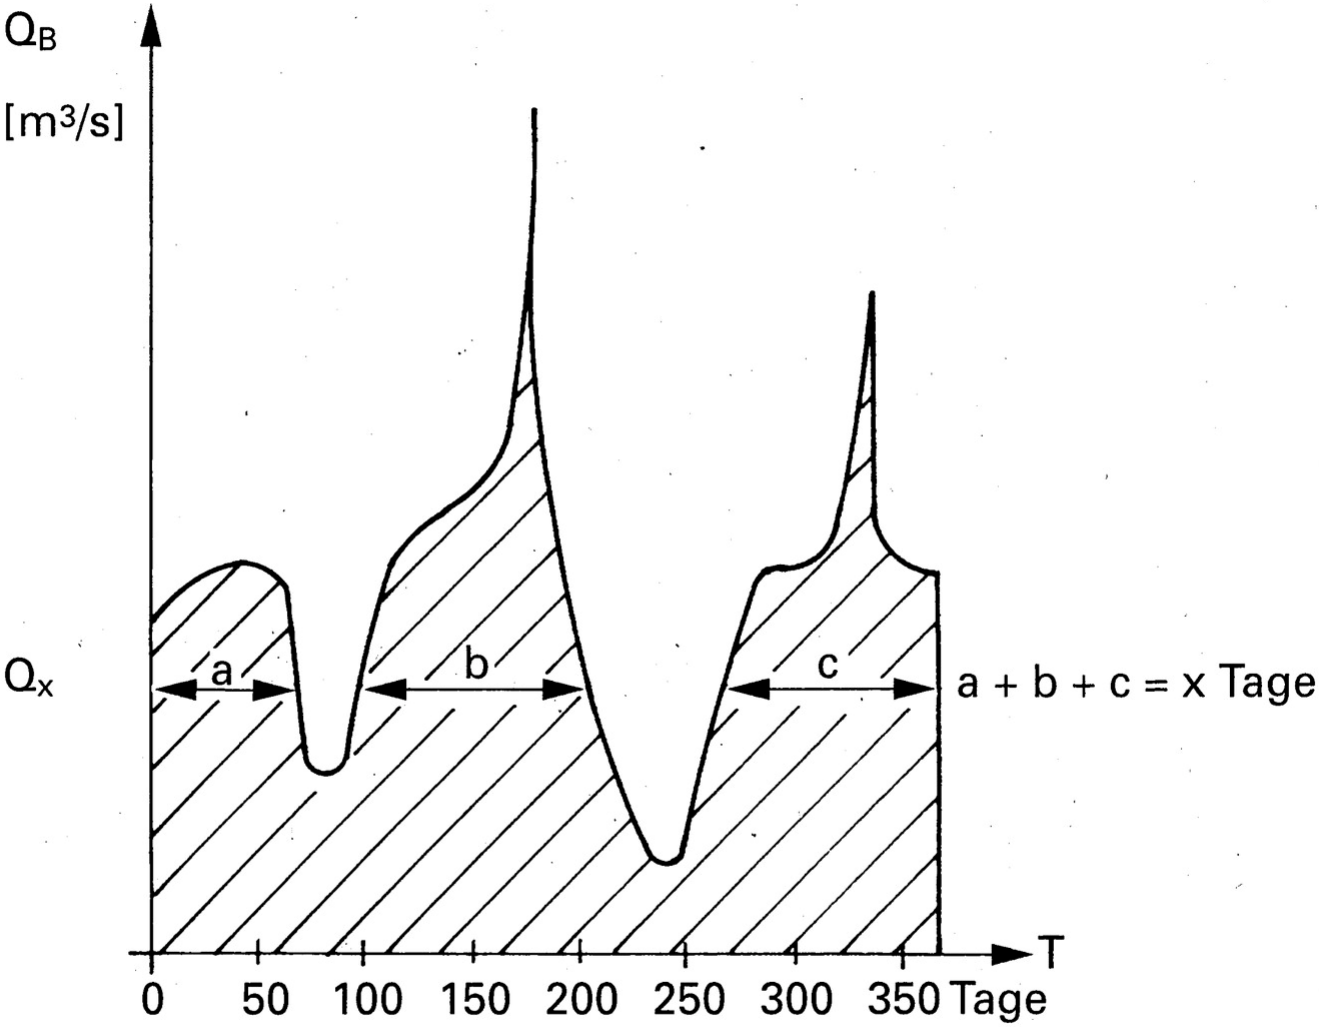
\includegraphics[width=0.95\textwidth, align=c]{images/Abflussganglinie.png}
    \end{center}
\end{minipage}

\vspace{0.25cm}



\subsection{Abflussdauerkurve}
Abfluss $Q_b$ in $\frac{m^3}{s}$ während eines Jahres (365 Tage), sortiert der Grösse nach\\
\begin{minipage}[c]{0.48\columnwidth}
    \begin{center}
        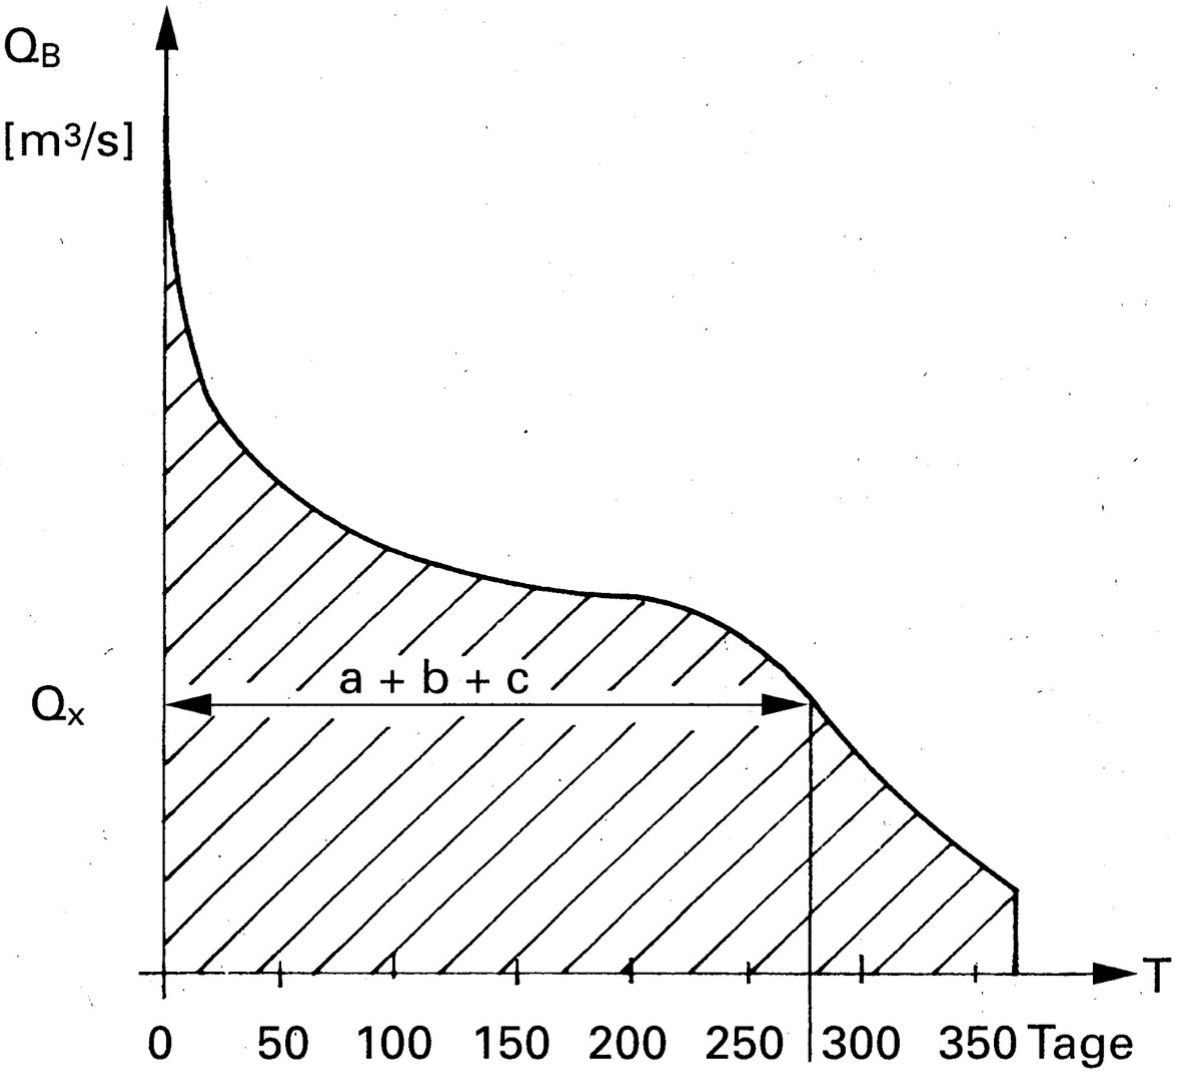
\includegraphics[width=0.95\textwidth, align=c]{images/Abflussdauerkurve.png}
    \end{center}
\end{minipage}

\vspace{0.25cm}

\textbf{Abfluss ist an 275 Tagen mindestens $Q_x$}



\subsection{Nutzwassermenge}
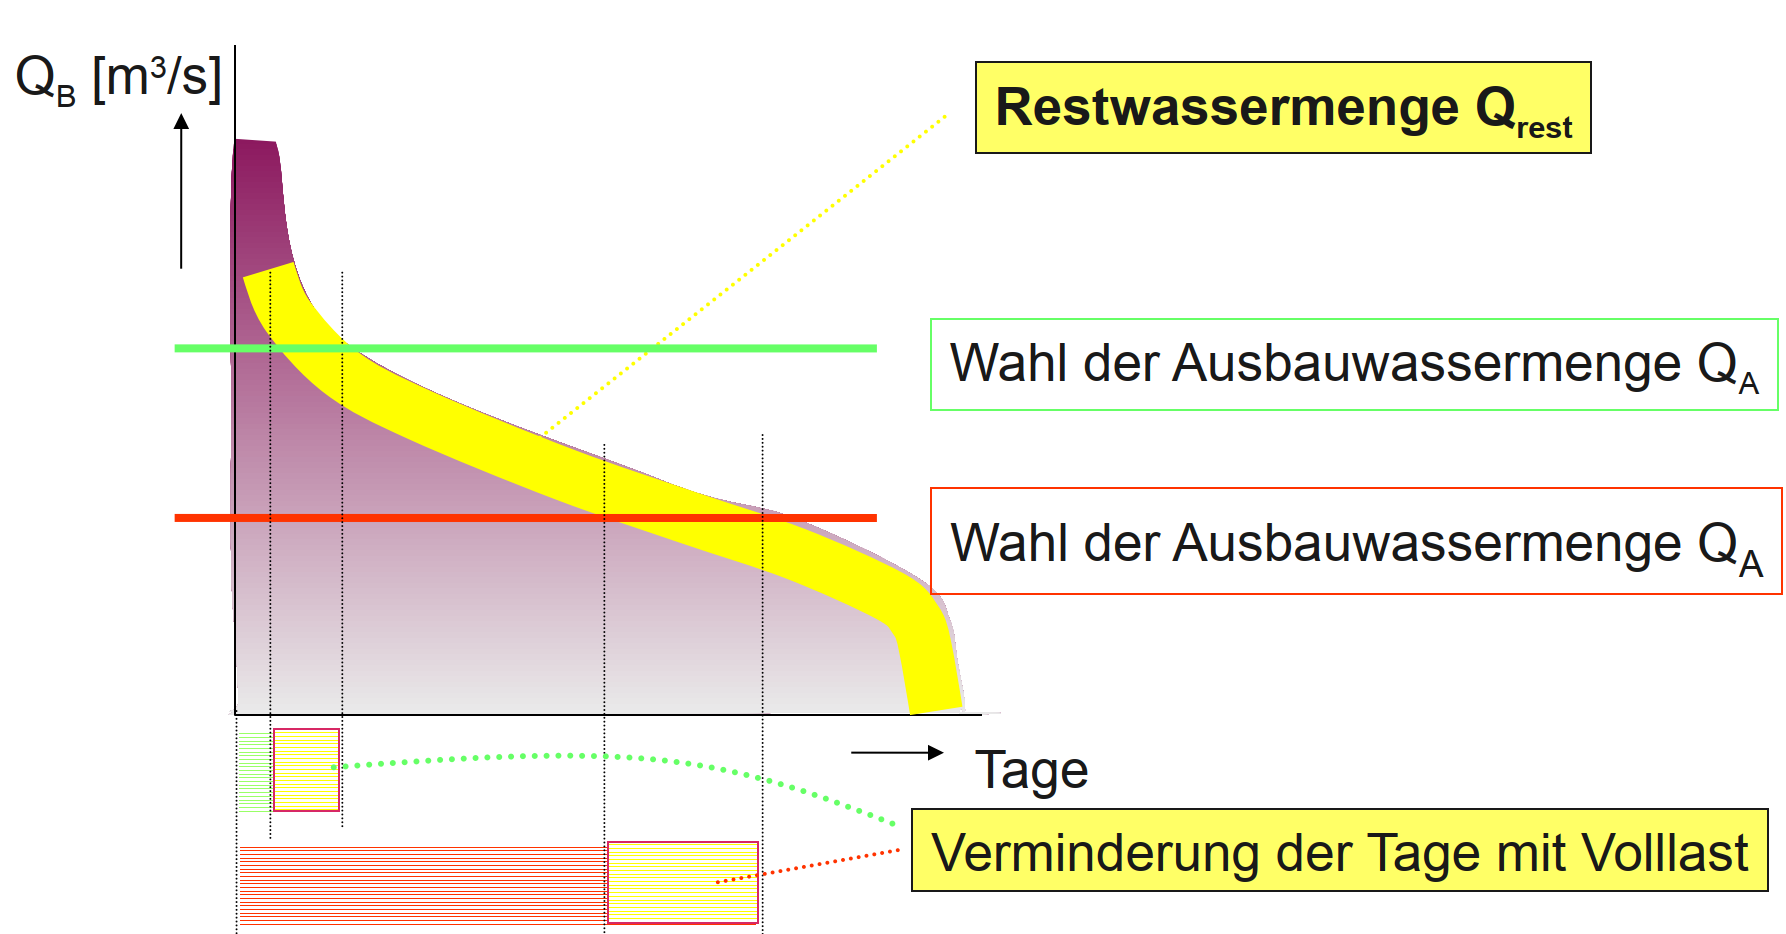
\includegraphics[width=0.95\columnwidth, align=c]{images/Nutzwassermenge.png}

\vspace{0.25cm}

$\boxed{Q_{Nutz} = Q_B - Q_{Rest}}$

\vspace{0.25cm}

\renewcommand{\arraystretch}{1.2} % Erhöht Zeilenhöhe für bessere Lesbarkeit
\begin{tabular}{@{} l p {6cm} l @{}}
    $[Q_{Nutz}]$    & Nutzwassermenge   \dotfill & $\frac{m^3}{s}$ \\
    $[Q_B]$         & Abflussmenge      \dotfill & $\frac{m^3}{s}$ \\
    $[Q_{Rest}]$    & Restwassermenge   \dotfill & $\frac{m^3}{s}$ \\
\end{tabular}
















        \newpage
\section{Wasserkraft}


\subsection{Kontinuitätsgleichung des Durchflusses}
\begin{center}
    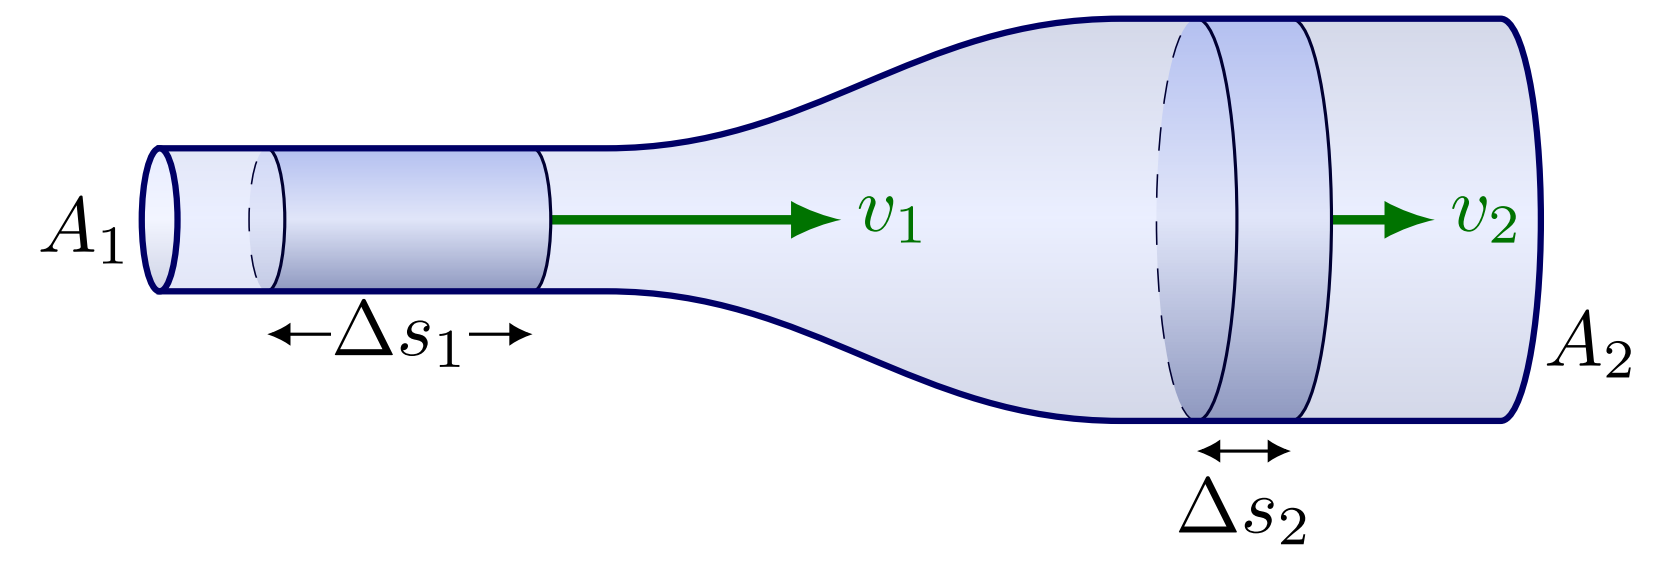
\includegraphics[width=0.9\columnwidth, align=c]{images/Kontinuitaet.png}
\end{center}

Die Kontinuitätsgleichung beschreibt die Erhaltung des Volumenstroms in einer strömenden Flüssigkeit:

\vspace{0.15cm}

$
\boxed{
    Q = A \cdot v 
} 
\quad
\boxed{
    Q_1 = Q_2 
} 
\quad
\boxed{
    A_1 \cdot v_1 = A_2 \cdot v_2
}
\quad
\boxed{
    Q = \dot{V} = \frac{\Delta V}{\Delta t} = \text{const} 
} 
$

\vspace{0.15cm}

\renewcommand{\arraystretch}{1.2} % Erhöht Zeilenhöhe für bessere Lesbarkeit
\begin{tabular}{@{} l p{6cm} l @{}}
    $[Q_x]$        & Durchflussrate                     \dotfill & $\mathrm{\frac{m^3}{s}}$ \\
    $[A_x]$        & Querschnittsfläche                 \dotfill & $\mathrm{m^2}$ \\
    $[v_x]$        & Fliessgeschwindigkeit              \dotfill & $\mathrm{\frac{m}{s}}$ \\
    $[\dot{V}]$    & Volumenstrom (Volumen pro Zeit)    \dotfill & $\mathrm{\frac{m^3}{s}}$ \\
    $[\Delta V]$   & Volumenänderung                    \dotfill & $\mathrm{m^3}$ \\
    $[\Delta t]$   & Zeitänderung                       \dotfill & $\mathrm{s}$ \\
\end{tabular}



\subsection{Bernoulli-Druck-Gleichung für Speicherwasserkraftwerke}

\begin{center}
    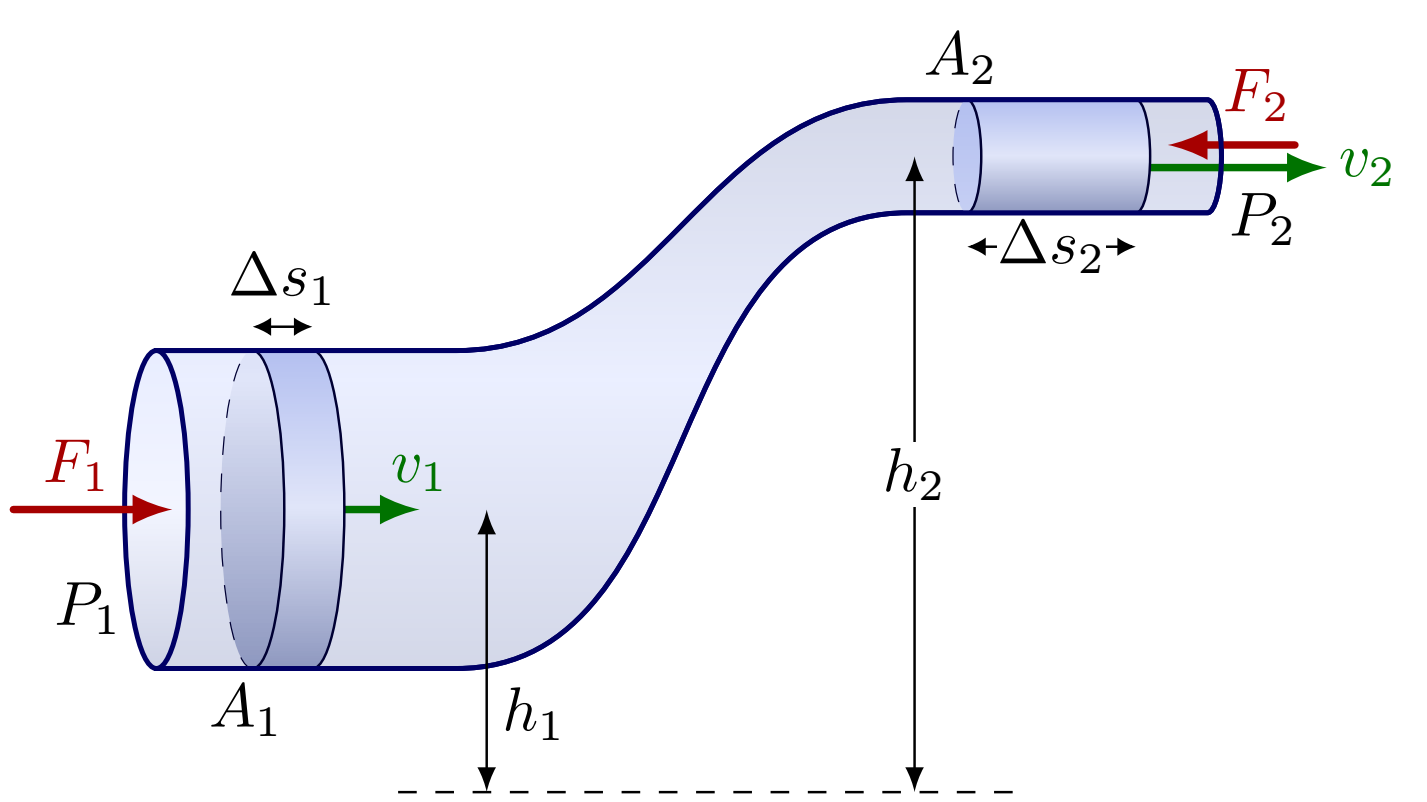
\includegraphics[width=0.9\columnwidth, align=c]{images/Bernoulli.png}
\end{center}

$\boxed{\frac{1}{2} \cdot \rho \cdot v^2 + \rho \cdot g \cdot z + p = \text{constant}}$

\vspace{0.15cm}

$
\boxed{
p_1 + \rho \cdot g \cdot h_1 + \frac{1}{2} \rho \cdot v_1^2 
= 
p_2 + \rho \cdot g \cdot h_2 + \frac{1}{2} \rho \cdot v_2^2
}
$

\vspace{0.15cm}

\renewcommand{\arraystretch}{1.2} % Erhöht Zeilenhöhe für bessere Lesbarkeit
\begin{tabular}{@{} l p {6cm} l @{}}
    $[\frac{1}{2} \rho v^2]$ & Kinetische Energie (je Kubikmeter) \dotfill & $\mathrm{\frac{J}{m^3}}$ \\
    $[\rho g z]$             & Potentielle Energie                 \dotfill & $\mathrm{\frac{J}{m^3}}$ \\
    $[p]$                    & Druckenergie                        \dotfill & $\mathrm{\frac{J}{m^3}}$ \\
\end{tabular}


\vspace{0.15cm}

$
\underbrace{p}_{A} + \underbrace{\rho g z}_{B} + \underbrace{\frac{1}{2}\rho v^2}_{C} = \underbrace{\text{constant}}_{D}
$


\subsection{Bernoulli-Höhen-Gleichung für Speicherwasserkraftwerke}

$\boxed{H = z + \frac{p}{\rho \cdot g} + \frac{v^2}{2 \cdot g} + \sum H_v}$

\vspace{0.15cm}

\renewcommand{\arraystretch}{1.2} % Erhöht Zeilenhöhe für bessere Lesbarkeit
\begin{tabular}{@{} l p {4cm} l @{}}
    $[H]$                           & Bruttogefälle                              \dotfill & $\mathrm{m}$ \\
    $[z]$                           & Höhenlage (potenzielle Energie)            \dotfill & $\mathrm{m}$ \\
    $[p]$                           & Druck                                      \dotfill & $\mathrm{Pa} = \mathrm{\frac{N}{m^2}}$ \\
    $[\rho]$                        & Dichte des Wassers                         \dotfill & $\mathrm{\frac{kg}{m^3}}$ \\
    $[g]$                           & Erdbeschleunigung                          \dotfill & $\mathrm{\frac{m}{s^2}}$ \\
    $[v]$                           & Geschwindigkeit                            \dotfill & $\mathrm{\frac{m}{s}}$ \\
    $\left[\frac{p}{\rho g}\right]$ & Druckhöhe                                  \dotfill & $\mathrm{m}$ \\
    $\left[\frac{v^2}{2g}\right]$   & Geschwindigkeitshöhe                       \dotfill & $\mathrm{m}$ \\
    $[\sum H_v]$                    & Hydraulische Energieverluste               \dotfill & $\mathrm{m}$ \\
\end{tabular}



\subsection{Örtliche Energieverluste}

$\boxed{h_v = \zeta \cdot \frac{v^2}{2g}}$

\vspace{0.15cm}

\renewcommand{\arraystretch}{1.2} % Erhöht Zeilenhöhe für bessere Lesbarkeit
\begin{tabular}{@{} l p {4cm} l @{}}
    $[h_v]$     & Örtliche Energieverlusthöhe   \dotfill & $\mathrm{m}$ \\
    $[\zeta]$   & Verlustbeiwert (dimensionslos) \dotfill & $-$ \\
    $[v]$       & Geschwindigkeit               \dotfill & $\mathrm{\frac{m}{s}}$ \\
    $[g]$       & Erdbeschleunigung             \dotfill & $\mathrm{\frac{m}{s^2}}$ \\
\end{tabular}



\subsection{Reibungsverluste (Formel von Strickler)}

$\boxed{h_{\text{v,r}} = \frac{v^2 \cdot L}{K_{St}^2 \cdot R_h^{4/3}}}$

\vspace{0.15cm}

\renewcommand{\arraystretch}{1.2} % Erhöht Zeilenhöhe für bessere Lesbarkeit
\begin{tabular}{@{} l p {4cm} l @{}}
    $[h_{\text{v,r}}]$  & Reibungsverlusthöhe           \dotfill & $\mathrm{m}$ \\
    $[v]$               & Strömungsgeschwindigkeit      \dotfill & $\mathrm{\frac{m}{s}}$ \\
    $[L]$               & Länge der Strömungsstrecke    \dotfill & $\mathrm{m}$ \\
    $[K_{St}]$          & Rauhigkeitsbeiwert nach Strickler \dotfill & $\mathrm{\frac{m^{1/3}}{s}}$ \\
    $[R_h]$             & Hydraulischer Radius          \dotfill & $\mathrm{m}$ \\
\end{tabular}



\subsubsection{Tabelle Rauhigkeitsbeiwert $K_{St}$ nach Strickler}
\begin{tabular}{|l|l|c|}
    \hline
    \textbf{Material} & \textbf{Zustand} & \textbf{$K_{St}$ [m$^{1/3}$/s]} \\
    \hline
    Stahl & neu & 75 \\
    \hline
    Stahl & schlechter Zustand, verrostet, verkrustet & 60 \\
    \hline
    Beton & glatt & 85 \\
    \hline
    Beton & rauh & 60 \\
    \hline
    PE, PVC &  & 100 \\
    \hline
\end{tabular}


\subsubsection{Hydraulischer Radius}

\begin{minipage}[c]{0.48\columnwidth}
    \myul{\textbf{Rechteckqueerschnitt}}\\
    \begin{center}
        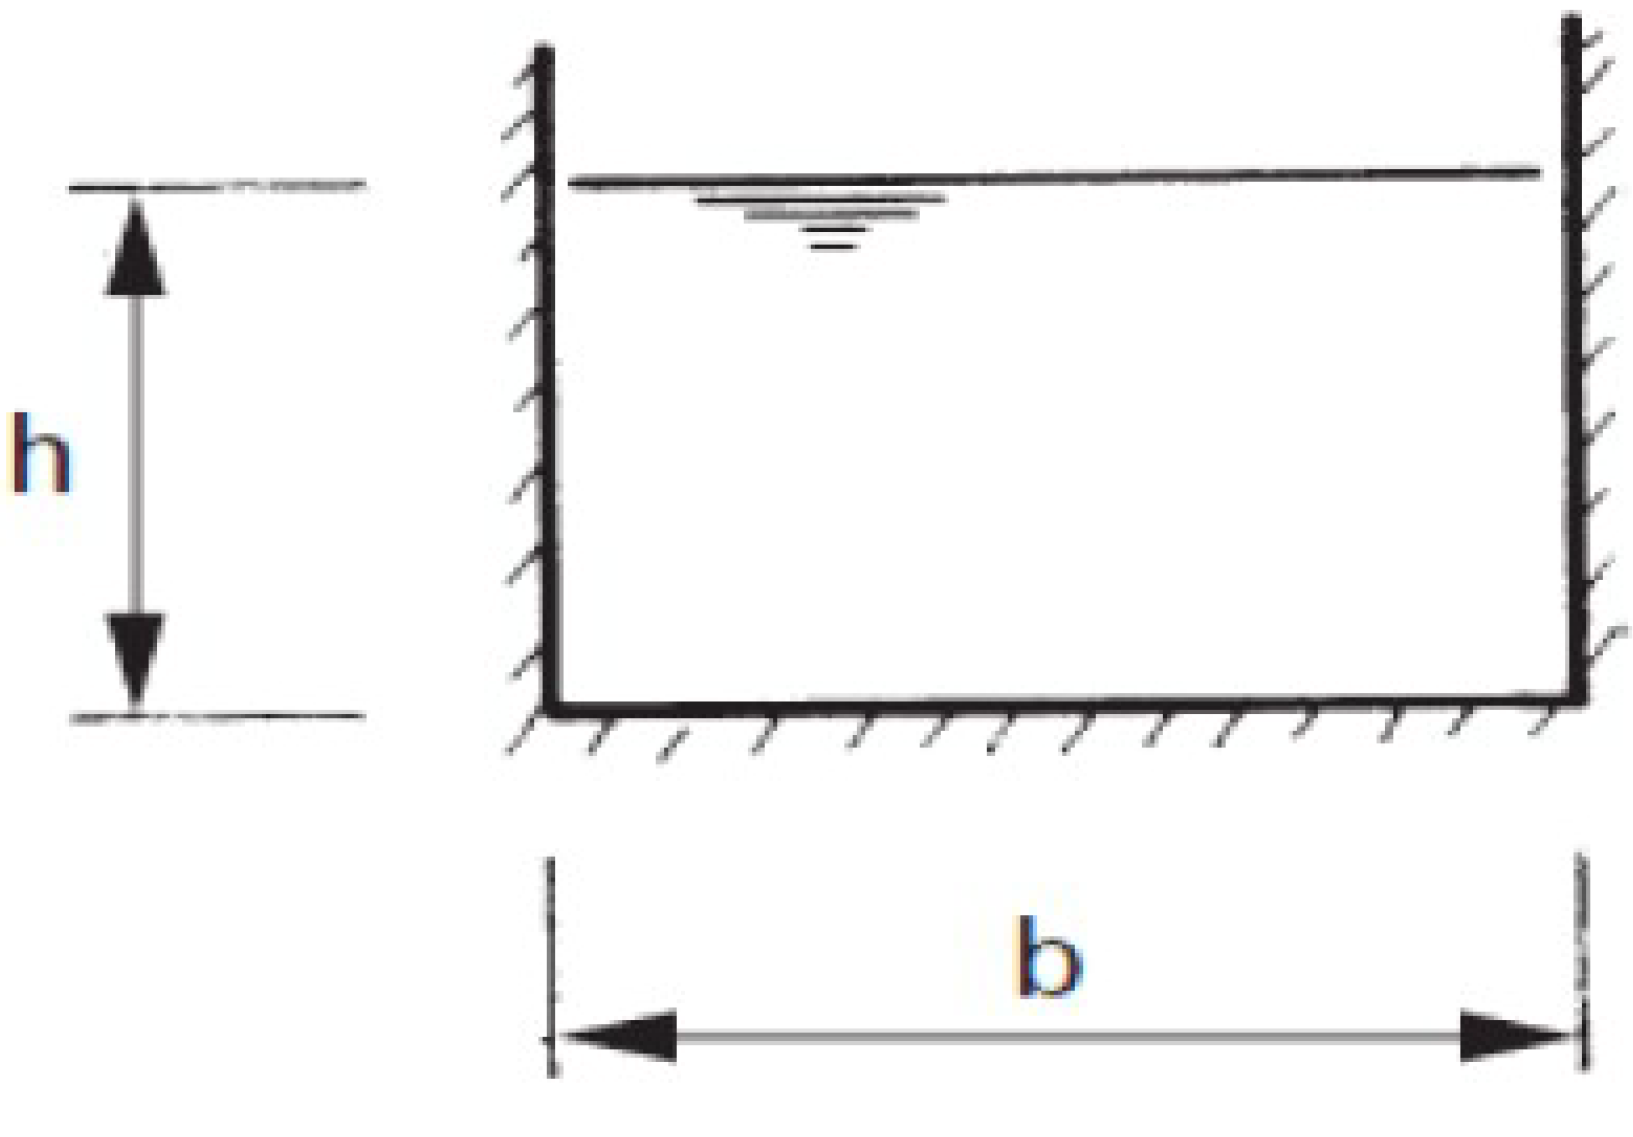
\includegraphics[width=0.9\textwidth, align=c]{images/Hydraulischer_Radius_Rechteck.png}
    \end{center}
\end{minipage}
\hfill
\vrule width 1pt % Vertikale Trennlinie mit 1pt Breite
\hfill
\begin{minipage}[c]{0.48\columnwidth}
    \myul{\textbf{Kreisqueerschnitt}}\\
    \begin{center}
        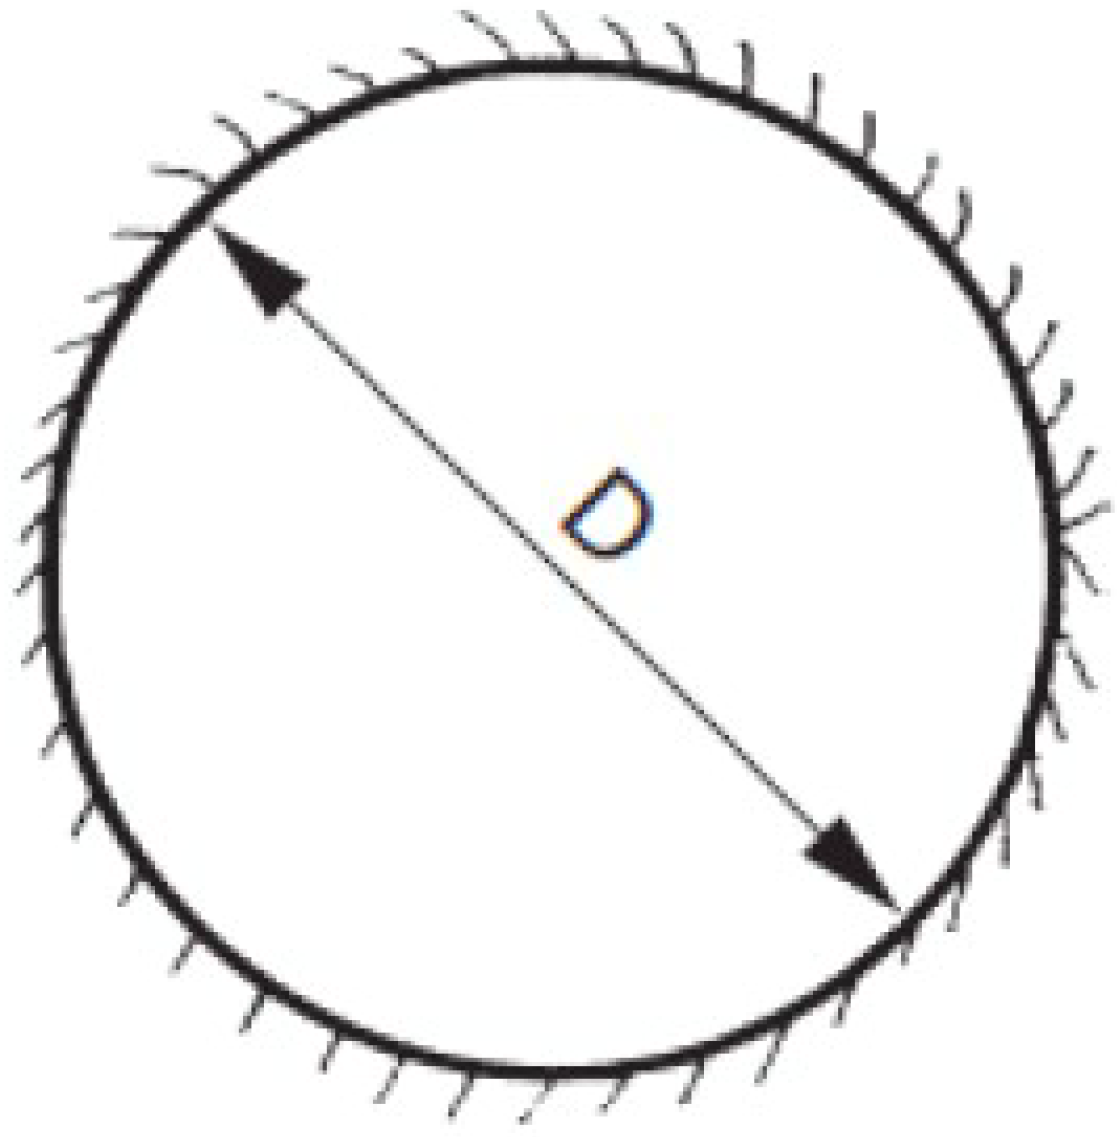
\includegraphics[width=0.65\textwidth, align=c]{images/Hydraulischer_Radius_Kreis.png}
    \end{center}
\end{minipage}

\vspace{0.25cm}

\begin{minipage}[c]{0.48\columnwidth}
    $\boxed{F = b \cdot h}$

    \vspace{0.15cm}

    $\boxed{P = b + 2 \cdot h}$

    \vspace{0.15cm}

    $\boxed{R_h = \frac{b \cdot h}{b + 2 \cdot h}}$ $\boxed{R_h = \frac{F}{P}}$
\end{minipage}
\hfill
\vrule width 1pt % Vertikale Trennlinie mit 1pt Breite
\hfill
\begin{minipage}[c]{0.48\columnwidth}
    $\boxed{F = \frac{D^2 \cdot \pi}{4}}$

    \vspace{0.15cm}

    $\boxed{P = D \cdot \pi}$

    \vspace{0.15cm}

    $\boxed{R_h = \frac{D}{4}}$ $\boxed{R_h = \frac{F}{P}}$
\end{minipage}

\vspace{0.15cm}

\renewcommand{\arraystretch}{1.2} % Erhöht Zeilenhöhe für bessere Lesbarkeit
\begin{tabular}{@{} l p {6cm} l @{}}
    $[F]$    & Abflussquerschnittsfläche         \dotfill & $\mathrm{m^2}$ \\
    $[P]$    & Benetzter Umfang                  \dotfill & $\mathrm{m}$ \\
    $[R_h]$  & Hydraulischer Radius              \dotfill & $\mathrm{m}$ \\
\end{tabular}





\subsection{Verlusthöhe durch Reibung}

$\boxed{h_{\text{v,r}} = \lambda \cdot \frac{L}{d_{\text{hy}}} \cdot \frac{v^2}{2 \cdot g} }
\quad
\boxed{h_{\text{v,r}} = \lambda \cdot \frac{L}{d_i} \cdot \frac{8 \cdot Q^2}{g \cdot \pi^2 \cdot d_i^4}}
\quad
\boxed{h_{\text{v,r}} = \frac{8 \cdot \lambda \cdot L \cdot Q^2}{g \cdot \pi^2 \cdot d_i^5}}$

\vspace{0.15cm}

\renewcommand{\arraystretch}{1.2} % Erhöht Zeilenhöhe für bessere Lesbarkeit
\begin{tabular}{@{} l p {6cm} l @{}}
    $[h_{\text{v,r}}]$  & Verlusthöhe durch Reibung      \dotfill & $\mathrm{m}$ \\
    $[L]$               & Länge                          \dotfill & $\mathrm{m}$ \\
    $[v_m]$             & Mittlere Geschwindigkeit       \dotfill & $\mathrm{\frac{m}{s}}$ \\
    $[Q]$               & Durchfluss                     \dotfill & $\mathrm{\frac{m^3}{s}}$ \\
    $[d_i]$             & Innendurchmesser               \dotfill & $\mathrm{m}$ \\
    $[d_{\text{hy}}]$   & Hydraulischer Durchmesser      \dotfill & $\mathrm{m}$ \\
    $[l_u]$             & Benetzter Umfang               \dotfill & $\mathrm{m}$ \\
    $[\lambda]$         & Verlustbeiwert                 \dotfill & $-$ \\
\end{tabular}


\vspace{0.15cm}

Zusammenhang des hydraulischen Durchmessers:

\vspace{0.15cm}

$
\boxed{d_{\text{hy}} = d_{\text{Kreisrohr}} = d_i = 4 \cdot R_{\text{hy}} = 4 \cdot \left(\frac{A}{l_u}\right)}
$



\subsection{Reynolds-Zahl $\text{Re}$}

Die Reynolds-Zahl $\text{Re}$ beschreibt das Verhältnis von Trägheitskräften zu Zähigkeitskräften in einer Strömung und wird wie folgt berechnet:

\vspace{0.15cm}

$\boxed{\text{Re} = \frac{v_m \cdot d_{\text{hy}}}{\nu}}$ \quad Bemerkung: $d_{\text{hy}} = d_{\text{Kreisrohr}} = d_i$

\vspace{0.15cm}

\renewcommand{\arraystretch}{1.2} % Erhöht Zeilenhöhe für bessere Lesbarkeit
\begin{tabular}{@{} l p {6cm} l @{}}
    $[\text{Re}]$     & Reynolds-Zahl (dimensionslos)                        \dotfill & $-$ \\
    $[v_m]$           & Mittlere Strömungsgeschwindigkeit                    \dotfill & $\mathrm{\frac{m}{s}}$ \\
    $[d_{\text{hy}}]$ & Hydraulischer Durchmesser                            \dotfill & $\mathrm{m}$ \\
    $[d_i]$           & Innendurchmesser (für Kreisrohr gleich $d_{\text{hy}}$) \dotfill & $\mathrm{m}$ \\
    $[\nu]$           & Kinematische Viskosität                              \dotfill & $\mathrm{\frac{m^2}{s}}$ \\
\end{tabular}



\newcolumn
\subsection{Verlustbeiwert }

$
\boxed{
\lambda = \left(\frac{1}{-2 \cdot \log \left( \frac{\varepsilon}{3{,}71} \right)}\right)^2
}
\quad
\boxed{
\lambda = \left(\frac{1}{-2 \cdot \log \left( \frac{k}{d_{hy} \cdot 3{,}71} \right)}\right)^2
}
$

\vspace{0.15cm}

\renewcommand{\arraystretch}{1.2}
\begin{tabular}{@{} l p{6cm} l @{}}
    $[\lambda]$ & Verlustbeiwert \dotfill & $-$ \\
    $[k]$ & äquivalente Rauheit \dotfill & mm \\
    $[d_{\text{hy}}]$ & Hydraulischer Durchmesser \dotfill & m \\
\end{tabular}



\subsection{Nettogefälle $H_n$}
$
\boxed{
H_n = H - \sum H_v - \frac{v^2}{2g}
}
\quad
\boxed{\sum H_v = C \cdot Q^2}
$

\vspace{0.15cm}

\renewcommand{\arraystretch}{1.2}
\begin{tabular}{@{} l p{6cm} l @{}}
    $[H_n]$       & Nettofallhöhe \dotfill & m \\
    $[H]$         & Bruttogefälle \dotfill & m \\
    $\left[\sum H_v\right]$ & Summe der hydraulischen Verluste \dotfill & m \\
    $[C]$         & Faktor bei Bestimmung der Verluste \dotfill & $\frac{\text{s}^{2}}{\text{m}^5}$ \\
    $[Q]$         & Volumenstrom \dotfill & $\frac{\text{m}^3}{\text{s}}$ \\
    $[v]$         & Strömungsgeschwindigkeit im Unterwasser \dotfill & $\frac{\text{m}}{\text{s}}$ \\
    $[g]$         & Erdbeschleunigung $g = 9{,}81$ \dotfill & $\frac{\text{m}}{\text{s}^2}$ \\
\end{tabular}



\subsection{Hydraulische Leistung $P_{\text{hyd}}$}

$
\boxed{P_{\text{hyd}} = \frac{m \cdot g \cdot H_n}{t} }
\quad
\boxed{P_{\text{hyd}} = \rho \cdot Q \cdot g \cdot H_n}
\quad
\boxed{\frac{\text{m}}{\text{t}} = \rho \cdot Q}
$

\vspace{0.15cm}

\renewcommand{\arraystretch}{1.2}
\begin{tabular}{@{} l p{6cm} l @{}}
    $[P_{\text{hyd}}]$  & Hydraulische Leistung \dotfill                & $\text{W}$ \\
    $[m]$               & Masse \dotfill                                & $\text{kg}$ \\
    $[g]$               & Erdbeschleunigung, $g = 9{,}81$ \dotfill      & $\frac{\text{m}}{\text{s}^2}$ \\
    $[H_n]$             & Nettofallhöhe \dotfill                        & $\text{m}$ \\
    $[t]$               & Zeit \dotfill                                & $\text{s}$ \\
    $[\rho]$            & Dichte des Wassers, $\rho = 1000$ \dotfill    & $\frac{\text{kg}}{\text{m}^3}$ \\
    $[Q]$               & Nutzwassermenge \dotfill                      & $\frac{\text{m}^3}{\text{s}}$\\ 
\end{tabular}



\subsection{Mechanische Leistung $P_{\text{mech}}$}

$
\boxed{P_{\text{mech}} = \eta_t \cdot P_{\text{hyd}}} 
\quad 
\boxed{P_{\text{mech}} = \eta_t \cdot \rho \cdot Q \cdot g \cdot H_n}
$

\vspace{0.15cm}

\renewcommand{\arraystretch}{1.2}
\begin{tabular}{@{} l p{7cm} l @{}}
    $[P_{\text{mech}}]$  & Mechanische Leistung an der Turbinen-Generator-Welle \dotfill & $\text{W}$ \\
    $[P_{\text{hyd}}]$   & Hydraulische Leistung \dotfill                               & $\text{W}$ \\
    $[\eta_t]$           & Turbinenwirkungsgrad \dotfill                               & $-$ \\
\end{tabular}



\subsection{Elektrische Leistung $P_{\text{el}}$}

$
\boxed{P_{\text{el}} = \eta_g \cdot P_{\text{mech}}} 
\quad 
\boxed{P_{\text{el}} = \eta_g \cdot \eta_t \cdot \rho \cdot Q \cdot g \cdot H_n}
$

\vspace{0.15cm}

\renewcommand{\arraystretch}{1.2}
\begin{tabular}{@{} l p{6cm} l @{}}
    $[P_{\text{el}}]$     & Elektrische Leistung an den Generatorklemmen \dotfill & $\text{W}$ \\
    $[P_{\text{mech}}]$   & Mechanische Leistung \dotfill                          & $\text{W}$ \\
    $[\eta_g]$            & Generatorwirkungsgrad \dotfill                         & $-$ \\
\end{tabular}



\subsection{Elektrische Energie $E$}

$
\boxed{E = \int P_{\text{el}} \cdot dt}
\quad
\boxed{E = \int \eta_g \cdot \eta_t \cdot Q \cdot H_n \cdot \rho \cdot g \cdot dt}
\quad
\boxed{E = \rho \cdot g \cdot \int \eta_g \cdot \eta_t \cdot Q \cdot H_n \cdot dt}
$

\vspace{0.15cm}

\renewcommand{\arraystretch}{1.2}
\begin{tabular}{@{} l p{6cm} l @{}}
    $[E]$               & Elektrische Energie \dotfill                           & $\text{Ws}$ \\
    $[P_{\text{el}}]$   & Elektrische Leistung \dotfill                          & $\text{W}$ \\
    $[\eta_g]$          & Generatorwirkungsgrad \dotfill                         & $-$ \\
    $[\eta_t]$          & Turbinenwirkungsgrad \dotfill                          & $-$ \\
    $[Q]$               & Nutzwassermenge \dotfill                               & $\frac{\text{m}^3}{\text{s}}$ \\
    $[H_n]$             & Nettofallhöhe \dotfill                                 & $\text{m}$ \\
    $[\rho]$            & Dichte des Wassers, $\rho = 1000$ \dotfill             & $\frac{\text{kg}}{\text{m}^3}$ \\
    $[g]$               & Erdbeschleunigung, $g = 9{,}81$ \dotfill               & $\frac{\text{m}}{\text{s}^2}$ \\
    $[t]$               & Zeit \dotfill                                           & $\text{s}$ \\
\end{tabular}

























































        %\newpage
\section{Wasserkraftwerk-Typen}

\subsection{Klassifizierung}

\begin{itemize}
    \item Laufwasserkraftwerke
    \item Mitteldruckanlagen
    \item Hochdruck- (Speicher-) Anlagen
    \item Pumpspeicherkraftwerke
    \item Gezeitenkraftwerke
    \item Wellenkraftwerke
    \item Wasserwirbelkraftwerke
\end{itemize}


\subsection{Einteilung nach technischen Aspekten}
\begin{itemize}
    \item \textbf{Laufwasserkraftwerke}
    \begin{itemize}
        \item Flusskraftwerke
        \begin{itemize}
            \item Blockbauweise
            \item Buchtenkraftwerke
            \item Zwillingsbauweise (beidseitige Anordnung)
            \item \dots
        \end{itemize}
        \item Ausleitungskraftwerke
    \end{itemize}
    
    \item \textbf{Speicherkraftwerke} mit natürlichem Zufluss
    \item \textbf{Pumpspeicherkraftwerke} (Speicherkraftwerke mit oder ohne natürlichem Zufluss)
    \item Gezeitenkraftwerke
    \item Wellenkraftwerke
\end{itemize}



\subsection{Einteilung nach energiewirtschaftlichen Aspekten}
\begin{itemize}
    \item Grundlastkraftwerke (häufig verwendet, Laufwasser, Speicher mit vielen Volllaststunden)
    \item Mittellastkraftwerke
    \item Spitzenlastkraftwerke (Speicher mit wenig Volllaststunden)
\end{itemize}



\subsection{Einteilung nach Betriebsart}
\begin{itemize}
    \item Verbundbetrieb (im Normalbetrieb alle Kraftwerke in der Schweiz)
    \item Inselbetrieb (Unabhängig vom Netz)
\end{itemize}



\subsection{Einteilung nach der installierten Leistung}
\begin{itemize}
    \item Kleinwasserkraftwerke (in der Regel kleiner 10 MW)
    \item Grosswasserkraftwerke (P > 10 MW)
\end{itemize}



\subsection{Einteilung nach wasserwirtschaftlichen Aspekten}
\begin{itemize}
    \item Wasserkraftwerke, die ausschliesslich elektrische Energie produzieren
    \item Wasserkraftanlagen für mehrere wasserwirtschaftliche Zielsetzungen (Mehrzweckanlagen, z.\,B. Trinkwasser)
\end{itemize}



\subsection{Wasserturbinen und Pumpen}

\begin{itemize}
    \item \textbf{Aktionsturbinen:} Arbeit aus kinetischer Energie-Differenz
    \begin{itemize}
        \item \textbf{Peltonturbinen}
    \end{itemize}

\item \textbf{Reaktionsturbinen:} Arbeit aus Druckdifferenz vor und nach Turbine
    \begin{itemize}
        \item Francisturbinen (spiralförmig)
        \item Kaplanturbinen (propellerförmig)
        \item Rohrturbinen
        \item Kreiselpumpen als Turbinen
    \end{itemize}
\end{itemize}



\subsection{Laufwasserkraftwerke LWK}

\begin{center}
    \includegraphics[width=0.95\columnwidth, align=c]{images/Laufwasserkraftwerke.png}
\end{center}

\begin{minipage}[c]{0.38\columnwidth}
    \begin{tabular}{c l}
        1 & Oberwasser \\ 
        2 & Unterwasser \\ 
        3 & Maschinenhaus \\
        4 & Stauwehr \\
        5 & Transformatoren \\
    \end{tabular}
\end{minipage}
\hfill
\begin{minipage}[c]{0.58\columnwidth}
    \begin{tabular}{c l}
        6 & Schaltanlage \\
        7 & Leitungen \\
        8 & Betriebsgebäude \\
        9 & Fischtreppe \\
        10 & Einrichtung für den Schiffstransport \\
    \end{tabular}
\end{minipage}



\subsection{LWK mit Kaplanturbinen Vertikal}

\begin{center}
    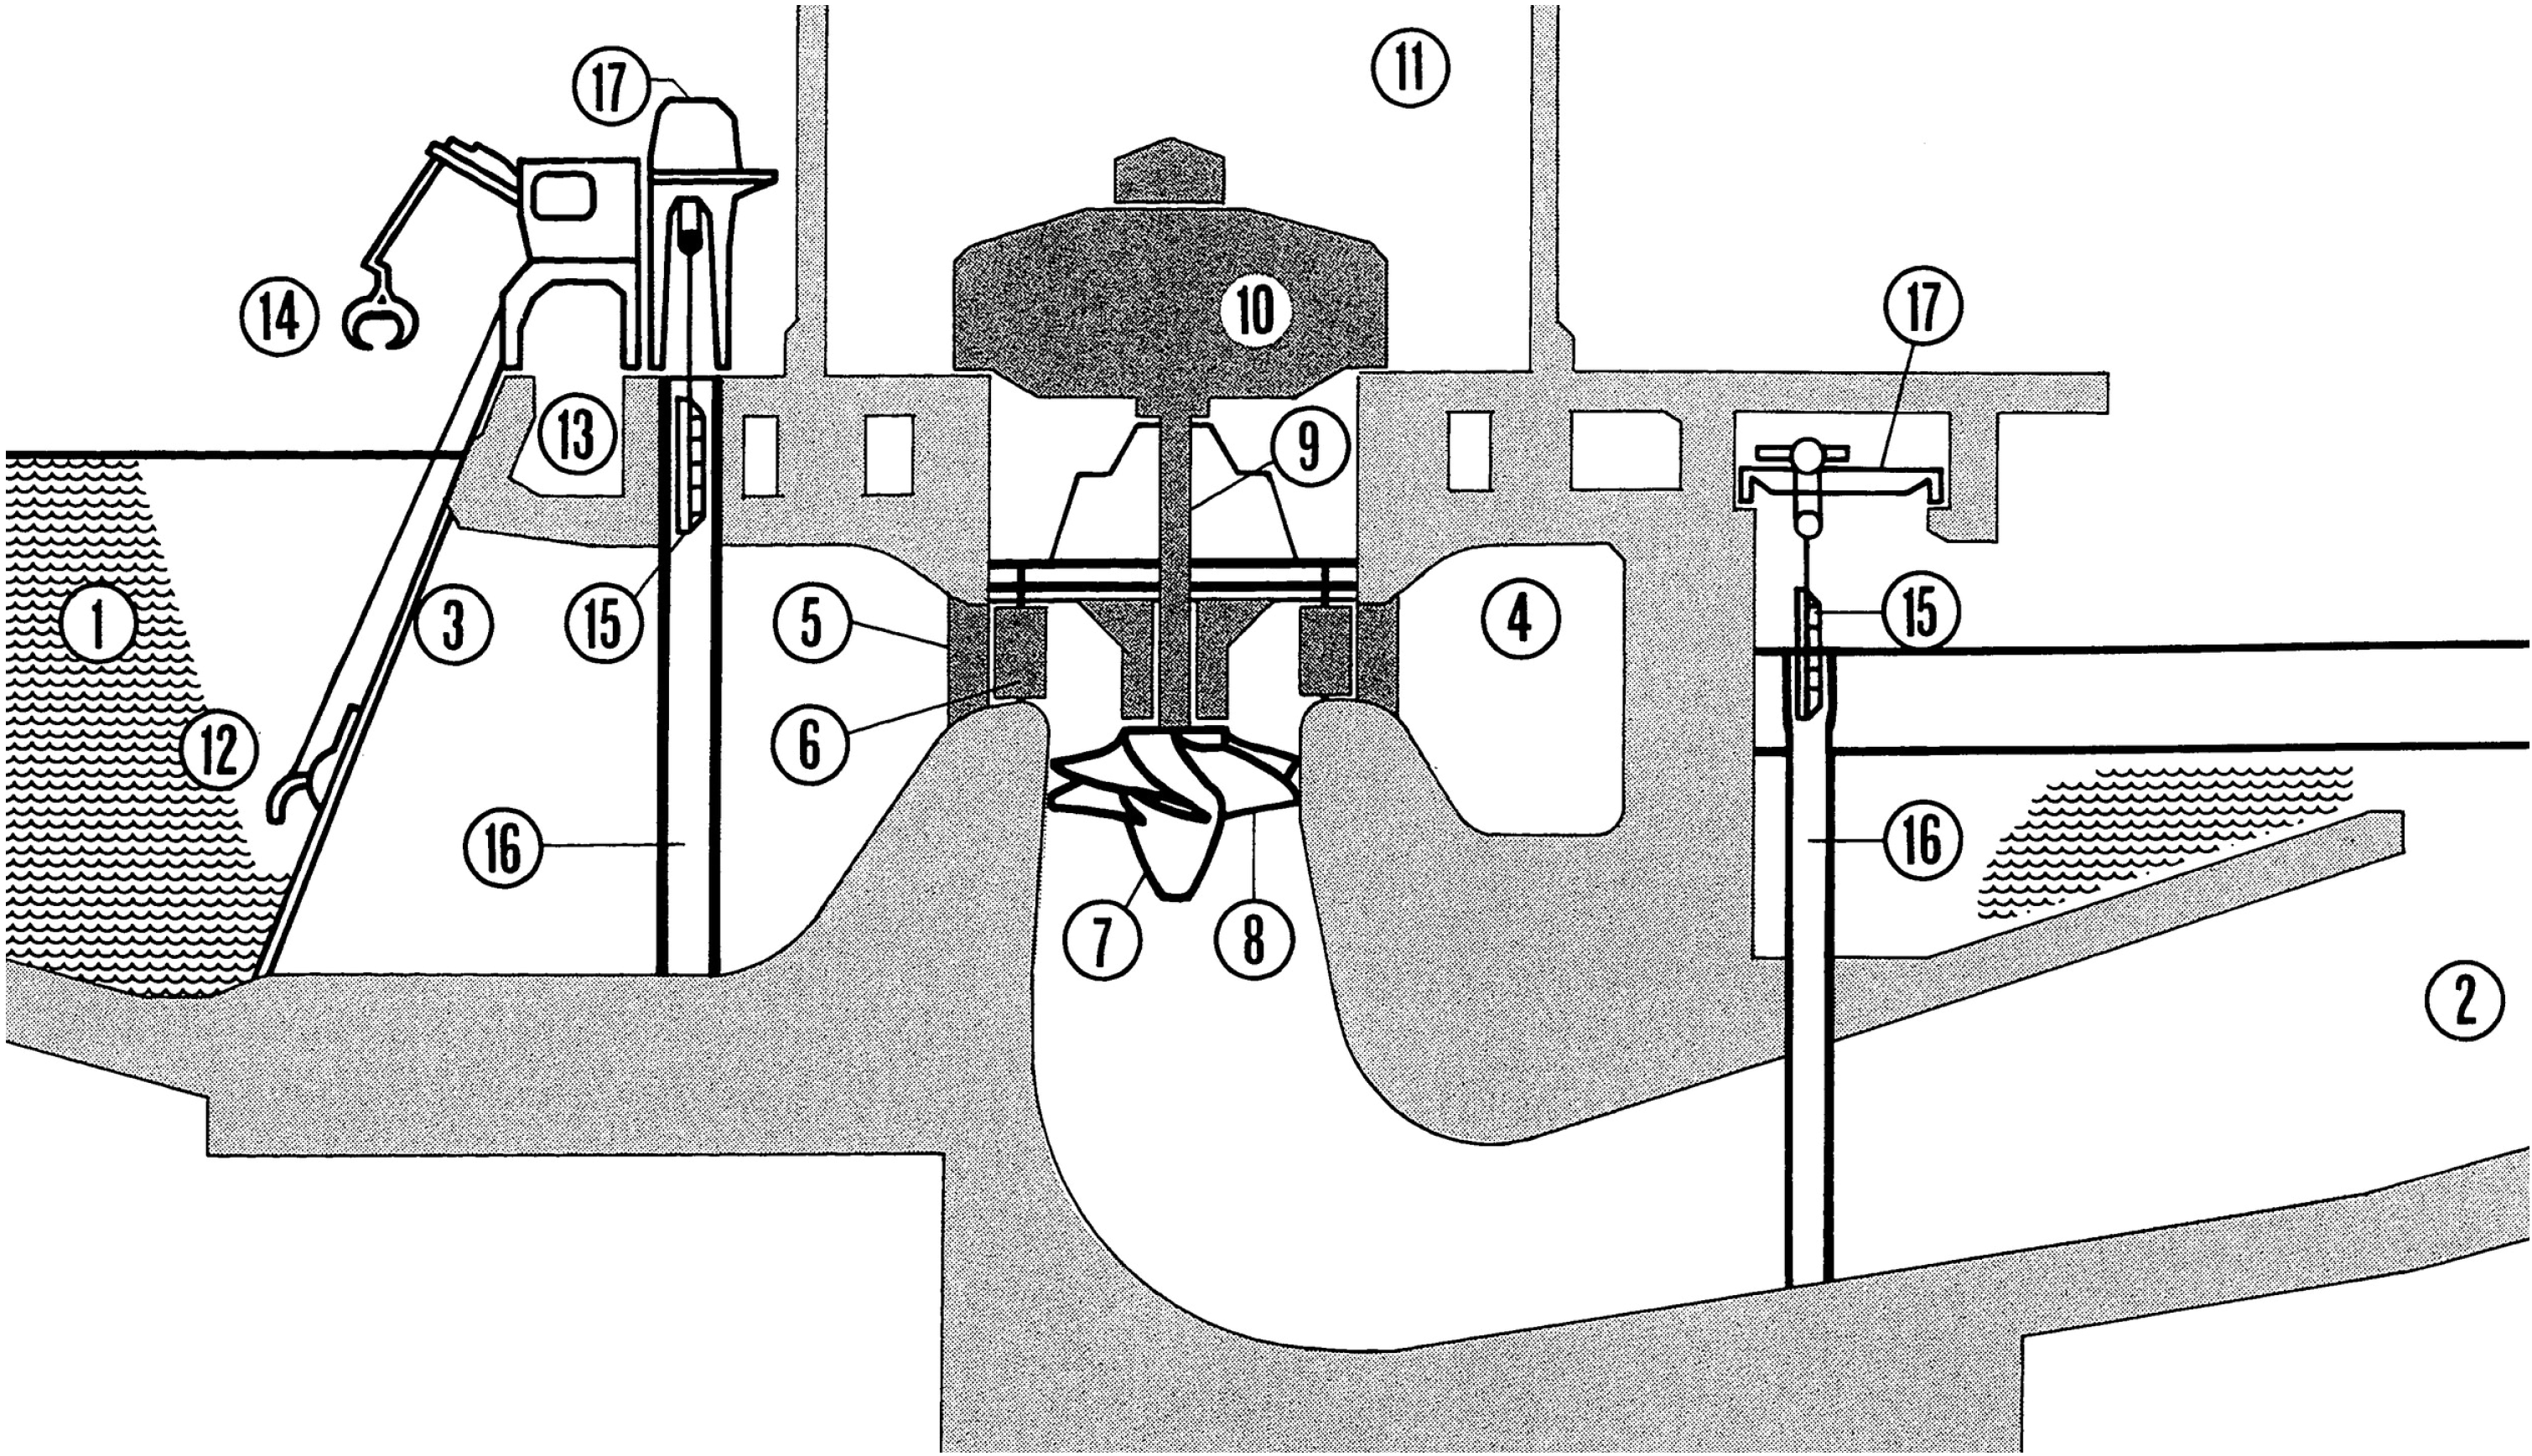
\includegraphics[width=0.95\columnwidth, align=c]{images/Laufwasserkraftwerke_Kaplanturbine_Vertikal.png}
\end{center}

\begin{minipage}[t]{0.38\columnwidth}
    \begin{tabular}{c l}
        1 & Oberwasser \\
        2 & Unterwasser \\
        3 & Rechen \\
        4 & Spirale \\
        5 & Stützschaufeln \\
        6 & Leitschaufeln \\
        7 & Laufrad \\
        8 & Laufradschaufeln \\
        9 & Saugrohr \\
    \end{tabular}
\end{minipage}
\hfill
\begin{minipage}[t]{0.58\columnwidth}
    \begin{tabular}{c l}
        10 & Generator \\
        11 & Maschinenhaus \\
        12 & Rechenreinigungsmaschine \\
        13 & Geschwemmselrinne \\
        14 & Zangengreifer \\
        15 & Dammbalken \\
        16 & Nuten für Dammbalken \\
        17 & Dammbalkenkran \\
           &  \\
    \end{tabular}
\end{minipage}



\subsection{LWK mit Kaplanturbinen Horizontal}

\begin{center}
    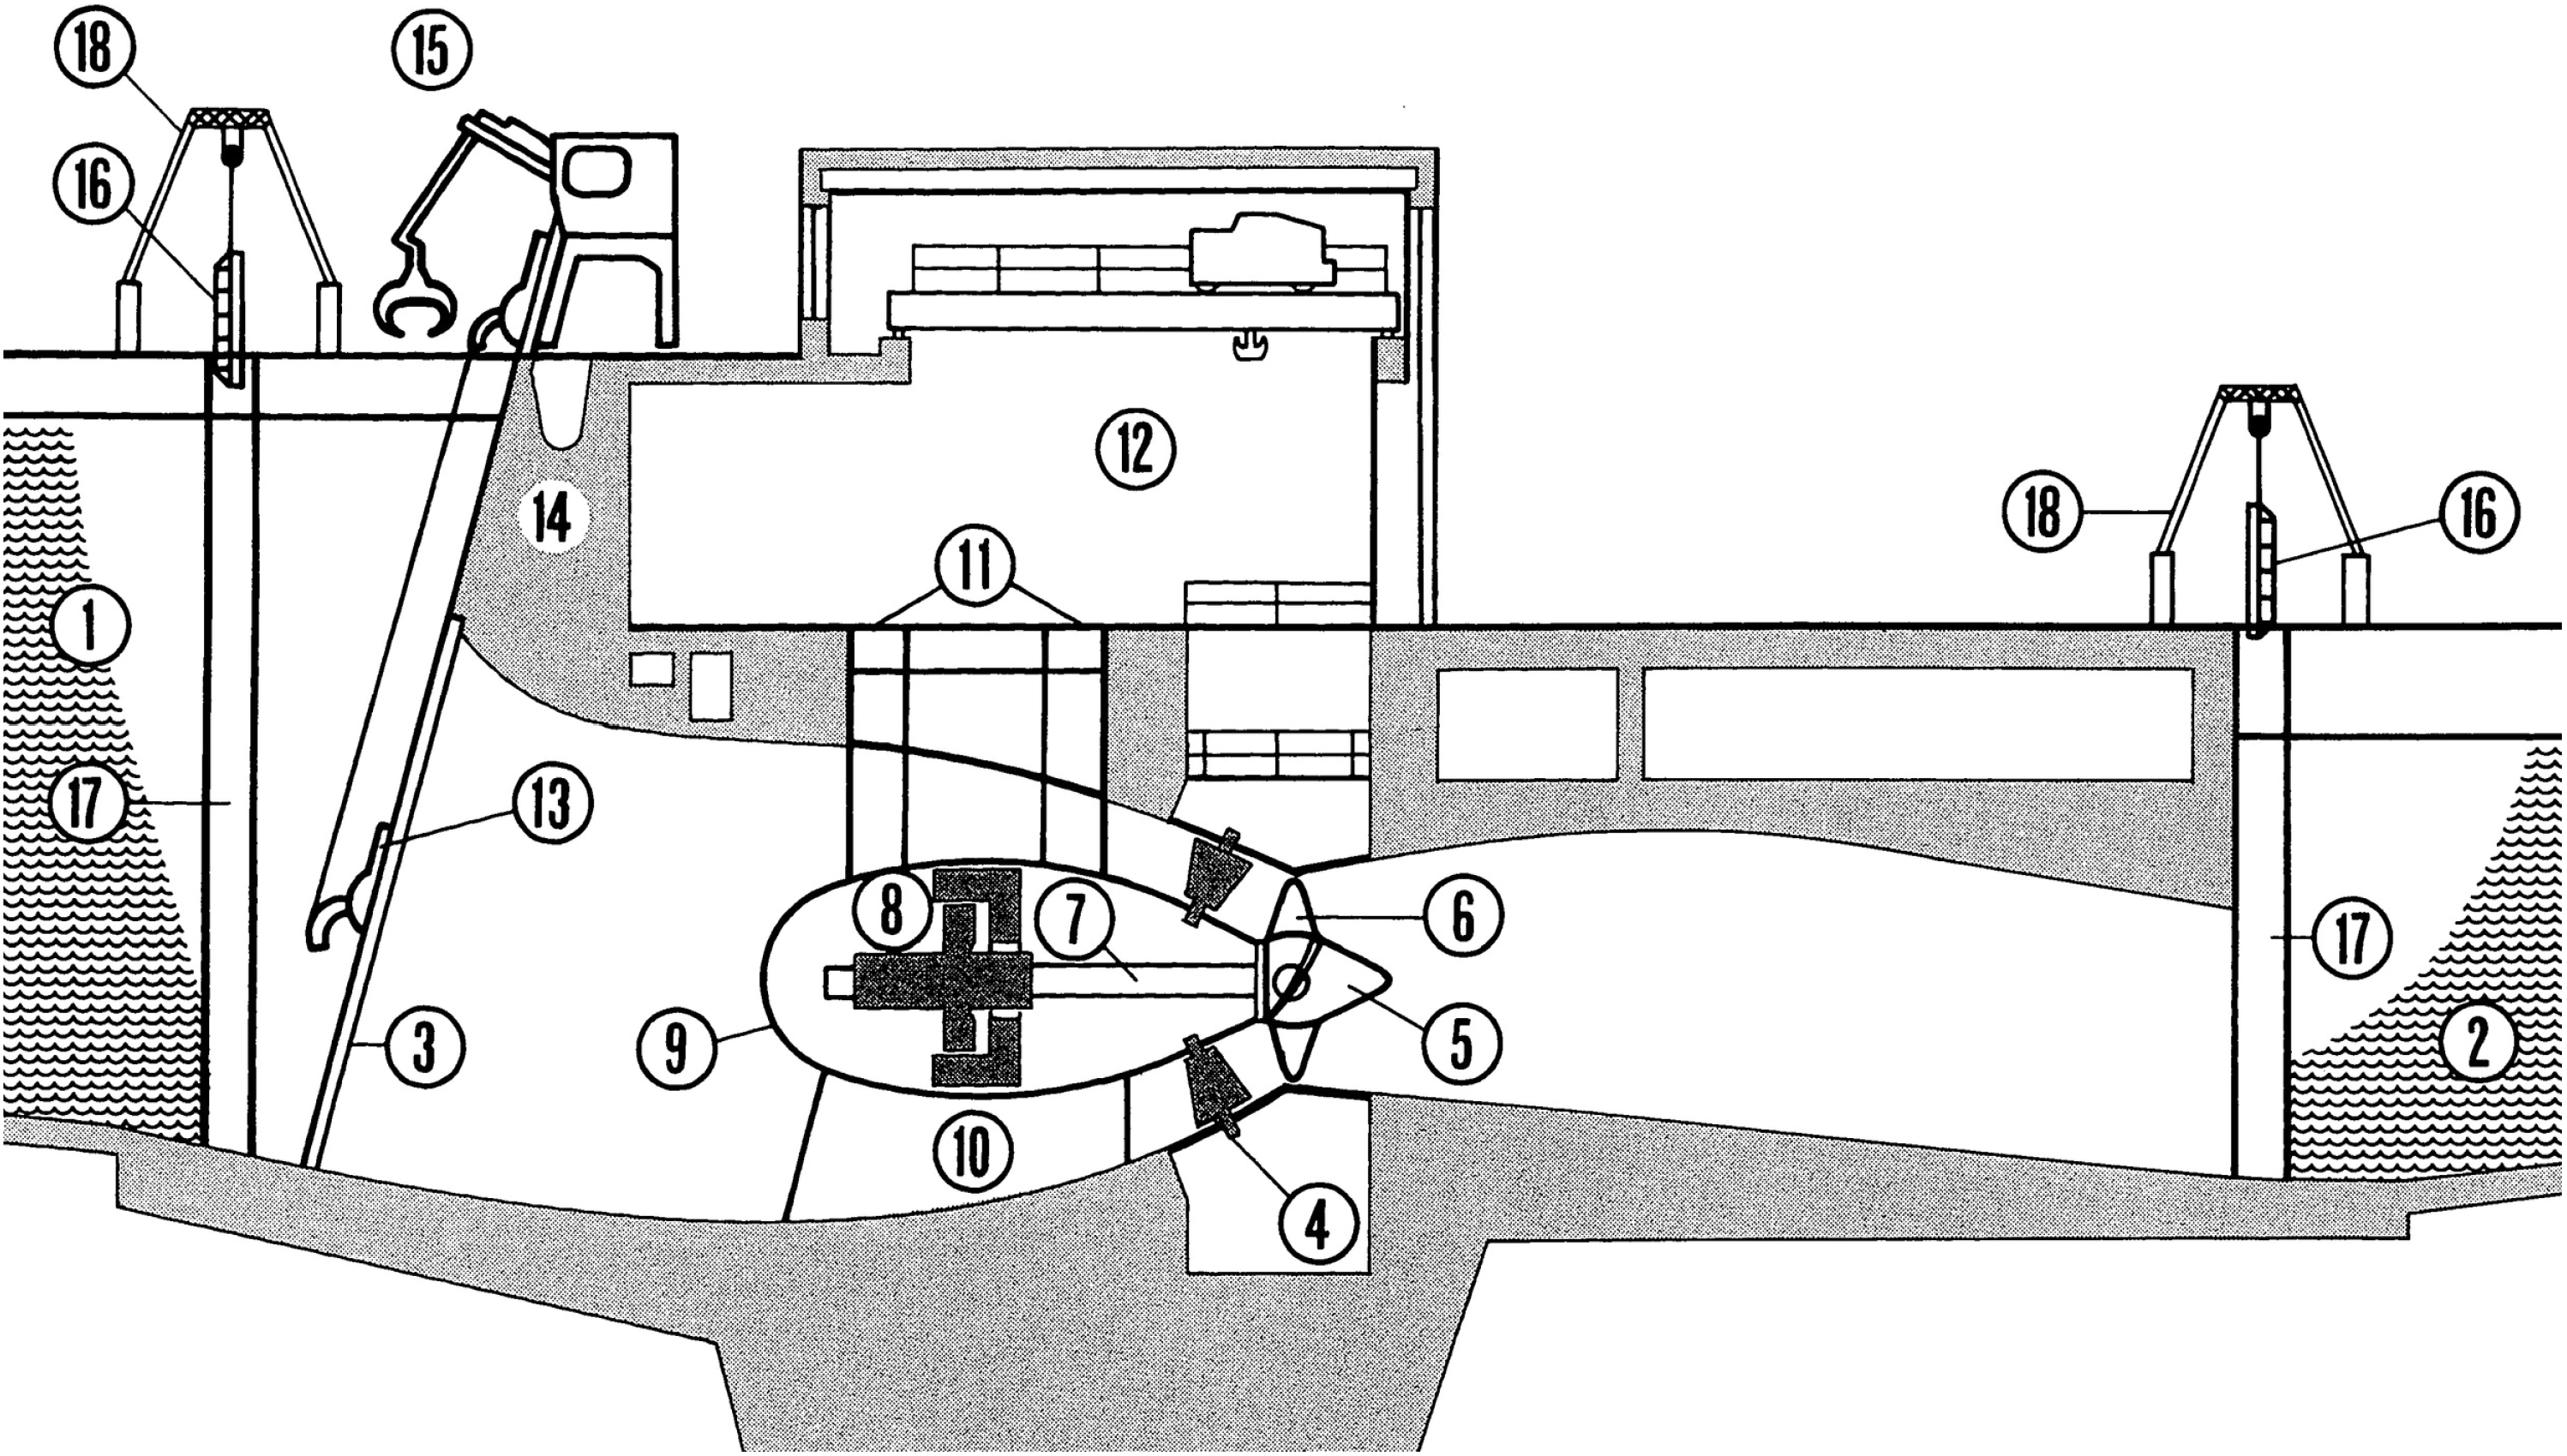
\includegraphics[width=0.95\columnwidth, align=c]{images/Laufwasserkraftwerke_Kaplanturbine_Horizontal.png}
\end{center}

\begin{minipage}[t]{0.38\columnwidth}
    \begin{tabular}{c l}
        1 & Oberwasser \\
        2 & Unterwasser \\
        3 & Rechen \\
        4 & Leitschaufeln \\
        5 & Laufrad \\
        6 & Laufradschaufeln \\
        7 & Turbinenwelle \\
        8 & Generator \\
        9 & Gehäuse \\
    \end{tabular}
\end{minipage}
\hfill
\begin{minipage}[t]{0.58\columnwidth}
    \begin{tabular}{c l}
        10 & Sockel \\
        11 & Einstiegsschächte \\
        12 & Maschinenhalle \\
        13 & Rechenreinigungsmaschine \\
        14 & Geschwemmselrinne \\
        15 & Zangengreifer \\
        16 & Dammbalken \\
        17 & Nuten für die Dammbalken \\
        18 & Dammbalkenkran \\
    \end{tabular}
\end{minipage}





































        %\newpage
\section{Turbinen Kenngrössen}
\subsection{Nettofallhöhe und Durchfluss}

\subsection{Hydraulische Leistung}

$\boxed{P_{\text{hyd}} = \rho \cdot Q \cdot g \cdot H_n}$

\renewcommand{\arraystretch}{1.2} % Erhöht Zeilenhöhe für bessere Lesbarkeit
\begin{tabular}{@{} l p {7cm} l @{}}
    $[P_{\text{hyd}}]$  & Hydraulische Leistung \dotfill & $W$ \\
    $[Q]$               & Nutzwassermenge \dotfill & $m^3/s$ \\
    $[H_n]$             & Nettofallhöhe \dotfill & $m$ \\
    $[\rho]$            & Dichte des Wassers ($\rho = 1000$) \dotfill & $\frac{kg}{m^3}$ \\
    $[g]$               & Erdbeschleunigung ($g = 9.81$) \dotfill & $\frac{m}{s^2}$ \\
\end{tabular}




\subsection{Mechanische Leistung an der Turbinenwelle}

$\boxed{P_{\text{mech}} = \omega \cdot M}$

\renewcommand{\arraystretch}{1.2} % Erhöht Zeilenhöhe für bessere Lesbarkeit
\begin{tabular}{@{} l p {6cm} l @{}}
    $[P_{\text{mech}}]$  & Mechanische Leistung   \dotfill & $W$ \\
    $[\omega]$           & Winkelgeschwindigkeit \dotfill & $\frac{\text{rad}}{s}$ \\
    $[M]$                & Drehmoment            \dotfill & $Nm$ \\
\end{tabular}


\subsection{Winkelgeschwindigkeit}

$\boxed{\omega = 2 \cdot \pi \cdot n}$

\renewcommand{\arraystretch}{1.2} % Erhöht Zeilenhöhe für bessere Lesbarkeit
\begin{tabular}{@{} l p {6cm} l @{}}
    $[\omega]$  & Winkelgeschwindigkeit \dotfill & $\frac{\text{rad}}{s}$ \\
    $[n]$       & Drehzahl              \dotfill & $\frac{1}{s}$ \\
\end{tabular}


\subsection{Betriebszustände der Maschinengruppe}
\textbf{(Maschinengruppe = Turbine/Pumpe + Generator/Motor)}

\begin{itemize}
    \item Inselbetrieb
    \item Parallelbetrieb, Verbundbetrieb
    \item Instationäre Vorgänge
    \begin{itemize}
        \item Anfahren und Abstellen
        \item Lastabwurf $\Rightarrow$ Überdrehzahl
    \end{itemize}
\end{itemize}

\textbf{Durchgangsdrehzahl $n_D$} (auch Schleuderdrehzahl genannt) $\Rightarrow$ höchste erreichbare Drehzahl ohne Last (z.B. bei Versagen des Generators)

Die Durchgangsdrehzahl ist eine Bemessungsgröße. Die Maschinengruppe darf bei der Durchgangsdrehzahl keinen Schaden erleiden.




















    \end{layout}
\end{document}
